
%\chapter{Epidemiological Modeling of News and Rumor on Twitter}
\chapter{Distinguish Real Movement from Rumor on Twitter}
%Event Classification based on Information Transition\\

% if you want to define paper specific  macros
% then put everthing between begingroup and endgroup
\begingroup
\newcommand{\score}{S}
\newcommand{\myalgo}{CoolAlgo}

%
%\begin{abstract}
%Characterizing information diffusion on social platforms like Twitter
%enables us to understand the properties of underlying media
%and model communication patterns. As Twitter gains
%in popularity, it has also become a venue to broadcast rumors and
%misinformation. We use epidemiological models to characterize
%information cascades in twitter resulting from both news and rumors.
%Specifically, we use the SEIZ enhanced epidemic
%model that explicitly recognizes skeptics to
%characterize eight events across the world and spanning
%a range of event types.
%We demonstrate that our approach is accurate at capturing diffusion in these
%events. Our approach can be
%fruitfully combined with other strategies that use content modeling
%and graph theoretic features to detect (and possibly disrupt) rumors.
%\end{abstract}

As social media (e.g., Twitter) continues to increase in popularity, it is becoming employed
as a social sensor into real-world mass movement event detection. Modeling and studying their adoption patterns gives us insight into investigate social and physical aspects of those events and precursors. This dissertation has presented several approaches and strategies with the goal of detecting and predicting mass movements and further inferring its causality, with given information mixed with real and rumor ones. Those include techniques to capture information propagation across multiple spaces, as well as a graph wavelet approach that broadens predictive capabilities to capture group abnormality within dynamic changing networks. Numerous forms of mass movements have been investigated and diverse aspects of modeling and detecting have been addressed. 

Using social media as indicator for real-word event detection is indeed helpful tool, however, they do possess limitations, perhaps most notably when applied to a specific event type, such as mass movement studied here. First, modeling protest-related topic propagation on networks is never trivial. One challenge is social protest propagation through online media can spread over large areas more quickly than traditional methods since users are geographically distributed, the other challenges include Mass protest information can be spread by multiple social medias and lot of paths, like word of mouth, TV and news broadcast. Second, detect the group abnormality on social media is not easy. One challenge is Twitter's user network embodies many subgraphs based on social ties which is dynamically changing the graph structures since users are active. The other challenge includes real world events are not only correlated with burst signals, but can also exhibit unusually low levels of activity in social networks. 
%Thereby how to define abnormality and capture those abnormality within dynamic changing networks?
Despite these restrictions, graph wavelet have in fact provided powerful capacity in capturing graph abnormality (considering burst behavior and absenteeism behavior), within dynamic changing networks.


A fundamental objective of this dissertation has been to model mass movement adoption behavior, and in doing so, several significant advantages are gained beyond the target. One contribution is the ability to model information propagation across multiple networks/spaces, and capture the propagation speed and possible propagation paths, which is demonstrated in Chapter 2. Another benefit that enhanced the mass movement detection is though group abnormality detection, as introduced in chapter 3. Graph wavelet provides appropriate definition of group abnormality which can cover both burst and absenteeism with different scales, thereby increasing the probability of capturing protest behaviors. Another by-product is the capability of quantify compartment transition dynamics using epidemic model SEIZ, and facilitate the development of screening criteria for distinguishing real movements from rumors happenings on Twitter, as demonstrated in Chapter 5.

Understanding information propagation over dynamic social network is highly-popular for addressing real-world problems in social network analysis. This dissertation analyzes several fundamental questions underlie the propagation-like processes, such as mass movement adoption, rumors transmission. These methodologies can be extended to other applications such as infectious diseases, public health, marketing, and so on. Given current advancements in information propagation, this is a revolutionary time for research in real-world applications using social network analysis. 





% comments from prilim
%\begin{itemize}
%\item North: lessons learned are?
%\item North: what does this say about the real phenomenon?
%\item North: help us learn about the semantics of the phenomenon
%\item North: why not detect rumors in other ways? Why not look at the source?
%\item CT: What's the relationship between rumors and absenteeism.. Spatial granularity can be common and can be harnessed. relationship between community and group abnormality,
%\item CT: climate keywords. Static keywords or dynamic keywords?
%\item Yang: why did u choose these particular techniques? no consistent theme across
%\item North: replace "4 problems in.." with a better title
%\item Feng: a treemap to connect the 4 topics
%\end{itemize}

\section{Related work}
Related work falls in three categories.
\paragraph{Information Diffusion}
Significant work has gone into research on information diffusion on
social media,
%Information diffusion in social networks is a well-researched topic, by
%both social scientists and data miners. One of the earlier ideas in this
%space was proposed by Everett Rogers in his theory ``Diffusion of
%Innovations" ~\cite{Rogers-diffusion1962} where he explained how, why, and
%at what rate do ideas spread through cultures. In recent years, online social networks have provided social scientists with
%an unprecedented amount of information, leading to a wide range of algorithmic
%approaches. There are some chapters focusing on the information diffusion across topics and time on Twitter, such as
e.g., see~\cite{Cha10measuringuser,Kwak:2010:TSN:1772690.1772751,Romero:2011:DMI:1963405.1963503,Yang_predictingthe}.
Recently, Matsubara etc.~\cite{matsubara2012rise}
conducted research on the rise and fall patterns of information diffusion, and managed to
capture the power-law fall pattern and periodicities inherent in such data.
Gomez-Rodriguez et al.~\cite{GomezRodriguez:2010:IND:1835804.1835933}
built a cascade transmission model to track cascading process taking place over a network; they traced overall blogs and news for a one-year period and found that the top 1000 media sites and blogs tend to have a
core-periphery structure.
%Kimura et al.\cite{Kimura:2009:EEI:1661445.1661772} discuss
%an approach to reduce the computational complexity of identifying most influential nodes in a large-scale network. They used two stochastic diffusion models and proposed a greedy algorithm on the basis of bond percolation and graph theory to reduce computational complexity. By modeling an email network as a graph, Wu et al \cite{WuFang2004b} found that the probability of a node forwarding a meme to a neighboring node decays as the graph distance between the node and the source increases. Gruhl et al. \cite{Gruhl04informationdiffusion} proposed a transmission graph to study information diffusion in the blogosphere, where they computed the probability that the topic will traverse the edge, following this they recomputed the posteriors and cycled through the process until convergence.
%%comprises a set of authors connected in a directed graph. Using the current version of the transmission graph, for each topic and each pair of authors they computed the probability that the topic will traverse the edge.
%
\paragraph{Epidemiological models}
Mathematical modeling of disease spread not only provides vital information about the propagation of the disease in a human network, but also offers insight into the strategies that can be used to control them.
%Kermack and McKendrick~\cite{Kermack1927Royal} study the effect of various factors that govern the spread of contagious epidemics in a population and are considered as one of the pioneers in this area. Later, Daley et al. \cite{Daley-nature-1964} suggested an analogy between the spread of disease and the dissemination of information and used epidemiological models to describe the growth and decay of rumor spreading processes. They divided the population into three mutually exclusive classes based on their dissemination of a rumor: have not heard it,
%are actively spreading it, and have stopped spreading the rumor.
%%This %division of the human population allowed them to apply the
%Kermack-McKendrick epidemic model to the propagation of a rumor.
The classification of the human population into different groups forms
the basic premise of using epidemiological models for modeling
information diffusion.
The two widely used such models are SIR (Susceptible, Infected, Recovered) and SIS (Susceptible, Infected, Susceptible) models. Newman et al.~\cite{PhysRevE.66.016128} showed that a large class of standard
epidemiological models, viz. the SIR models, can be solved exactly on a wide variety of networks, and confirmed the correctness of solutions with numerical simulations of SIR epidemics on networks. Kimura et al.~\cite{Kimura:2009:EEI:1661445.1661772} proposed the application
of the SIS model to study information diffusion where the nodes can be activated multiple times.
%In our chapter, we also applied SIS model for news and rumor spreading over Twitter.
%They created a layered graph from the social network where layers gets added on top of each other and then apply bond percolation with a pruning strategy with an intent to lower the computational complexity of the SIS model.
% \cite{Alison2010-Society} use a modified SIS model to prove emotions spreads very much like an infectious disease.
%tried to evaluate the spread of long-term emotional states across a social network using a modified SIS model which included the possibility of spontaneous infection. They were able to provide evidence that emotions spreads very much like an infectious disease.
Zhao et al.~\cite{RePEc:eee:phsmap:v:392:y:2013:i:4:p:987-994} proposed an SIHR (Spreaders, Ignorants, Hibernators, Removed) rumor spreading model,
with forgetting and remembering mechanisms to simulate rumor spreading in inhomogeneous networks.
Xiong et al.~\cite{Xiong20122103} proposed a diffusion model with four different states: susceptible, contacted, infected, and refractory (SCIR) to identify the threshold value of the spreading rate approaches almost zero.
%They study information diffusion on Twitter using the retweeting mechanism.
%There were able to identify that the threshold value of the spreading rate approaches almost zero and that the degree-based density of infected agents increases with the degree monotonously.
Bettencourt et al.~\cite{powerofgoodidea:2006} proposed the SEIZ (susceptible, exposed, infected, skeptic) model to capture the adoption of Feynman diagrams by using the publication counts after World War II. They extract the general features for idea spreading and estimate the idea adoption process. Their result showed that
the SEIZ model can fit the long term idea adoption process with reasonable error, but does not demonstrate whether this model can be applied on large scale datasets, or whether can be applied on Twitter, where the story unfolds in real-time.

\paragraph{Rumor modeling}
As far as we know, Daley~\cite{Daley-nature-1964} first proposed the similarity between epidemics and rumors using mathematical analysis. Some researchers have studied rumor propagation modeling in different network topologies~\cite{nekovee2007theory,zanette2002dynamics}; however,
they do not provide any discussion of propagation differences between news and rumors.
Shah et al.~\cite{shah2011rumors} detect rumor sources in network using maximum likelihood modeling.
In~\cite{budak2011limiting}, Budak et al. prove that minimizing the spread of the misinformation (i.e., rumors)
in social networks is an NP-hard problem and also provide
a greedy approximate solution. Castillo et al.~\cite{castillo2011information} delve into twitter content modeling, such as sentiment analysis and
hashtags to identify rumors, while Qazvinian et al.~\cite{qazvinian2011rumor} try to address this issue using broader linguistic methods,
to learn possible features of rumor and determine whether a twitter
user believes a rumor or not. More related work appears
in~\cite{Isham-physica-2009,PhysRevE.81.056102}. Our goal is to develop an understanding of
these processes using diffusion models.
%
%Trpevski et al. \cite{PhysRevE.81.056102} used the SIS model to study how two different rumors propagate in a network, Zhou et al.~\cite{Zhou2007458} studied rumor propagation in complex networks using the SIR model, while Zhao et al \cite{RePEc:eee:phsmap:v:392:y:2013:i:4:p:987-994} proposed a modified SIR model where they assumed that ignorants will inevitably change their status to either spreaders or stiflers after getting contacted by the spreaders, and Ishama et al. \cite{Isham-physica-2009} try to find the final size of a rumor on a homogeneous network using the stochastic SIR epidemic model, where they applied embedded Markov chain techniques to derive a set of equations that can be solved numerically to identify the spread of a rumor.
%These two rumors are initiated with different probabilities of acceptance. They found that one of
%the rumors is typically more dominant in the network compared to other.
%However, all their research works are based on simulation modeling whereas our work here are trying to model actual news and rumor propagation on Twitter.
%
% Compared with our approach, we are trying to identify rumors from diffusion properties, via an extended epidemic model SEIZ \cite{powerofgoodidea:2006}, from which we can get a ratio of the rate at which people get exposed (and not believe) to the rate at which people move from exposed to belief. We think the different distributions of the max ratio might shed some light on news and rumor detection. while they didn't address the dynamic rumor propagation models in twitter.
%\narenc{is it skeptics or is it skeptic? Pick one and stick with it.}

%\narenc{The related work in general is very poorly written. It reads like this:
%
%A et al.. did this.
%B et al. did this.
%C et al. did this.
%
%There is no structure, no organization. You need a good story. The sentences
%have to be more tightly linked. Look at some of my chapters to get
%an idea. You don't need 1 sentence for each chapter. You can group chapters
%further and cite them together. For instance: Some chapters [CITE1, CITE2]
%take the approach of WHATEVER. The whole related work must be in 1 page
%but without losing any citations. }

%\narenc{Looks like this is not just
%tweet news dataset. It contains both news and rumors. And it is not
%a dataset. It is many datasets. You can just call it Tweet datasets studied
%in this chapter. Replace 'Real' by 'Type' so that the types are
%News and Rumor, not True and Rumor. Remove Lang, Collection columns.}


\section{Datasets}

\begin{table*}[!htp]
\tiny
\caption{Twitter datasets studied in this chapter.} % title of Table
\vspace{0.5em}
\centering % used for centering table
\begin{tabular}{| p{0.3cm} | p{1.2cm} | p{1.4cm} | p{1.6cm} | p{0.8cm} | p{1.1cm} | p{0.8cm} | p{1.4cm} | p{4.2cm} | }
\hline %inserts double horizontal lines
\textbf{No.}& \textbf{Dataset} & \textbf{Date}  & \textbf{Area} & \textbf{Type} & \textbf{Country} & \textbf{\#Tweets} & \textbf{Response ratio} & \textbf{Keywords \& Hashtag}  \\ [1ex] % inserts table
%heading
\hline % inserts single horizontal line
1& Boston & 04-15-2013&  terrorism& news & USA &  501259 &68.3\% & Marathon, (\#)bostonmarathon \\[1ex]
\hline
2&  Pope & 02-11-2013 &religion&news & Vatican & 31365 &56.75\% &Pope, (\#)Benedict \\[1ex]
\hline
3& Amuay &08-25-2012&  accident &news & Venezuela&49015 &62.89\% &Amuay, refinery, explosion \\[1ex]
\hline
4& Michelle &02-24-2013&  entertainment & news & USA& 3762& 54.45\% &Michelle Obama, Oscars   \\[1ex]
\hline
5& Obama & 04-23-2013&  politics& rumor & USA & 791&46.14\% &White House, explosions    \\[1ex]
\hline
6& Doomsday & 12-21-2012&  mythology& rumor & Global &11833 &52.19\%& Doomsday, Mayan, doom  \\[1ex]
\hline
7& Castro & 10-16-2012&  politics & rumor & Cuba & 3862& 54.45\% &Fidel Castro, Dr. Marquina \\ [1ex]
\hline
8& Riot & 09-05-2012& crime & rumor & Mexico &4631& 47.17\% & Antorcha Campesina, Nezahualcoyotl\\ [1ex]
\hline
\end{tabular}
\label{table:story-intro} % is used to refer this table in the text
\end{table*}


We focus on twitter datasets that have reliable coverage of the
events being studied; the volume of tweets ranges from as low as
791 to nearly three orders of magnitude greater.
As described in Table~\ref{table:story-intro},
the news and rumors studied were drawn from a variety of
regions and across a diversity of topics.
Data collection was aimed at gathering tweets highly related to the events
under study. We employed customized sets of keywords and hashtags pertaining
to each incident.
%%%%%%%%%%%%%%%%% I removed this sentence, since I did not apply geolocation algorithms.  %%%%%%%%%%%%%%%%%%
%In addition, since our stories spanned many geographic regions, we employed geolocation algorithms that inspect either (latitude, longitude) coordinates or other user profile information.
Finally, date range restrictions were used to define relevant tweets for
each event. It is also pertinent to note that the tweets analyzed spanned
a variety of languages: English, Spanish, Italian, and Portuguese.

%This section describes the twitter data sets which were used for our analysis. Since there are millions of news related tweets published every day on Twitter, we selected only the ones which met the following criteria: (1) the volume of tweets related to the event should be more than 2000. (2) Reliable news sources have mentioned the news/rumor in their tweets. In this chapter, we used eight news events for our analysis which are described in table , Out of the eight news events five were true news and the rest three were rumors. The nature of the news events were determined by confirming with the appropriate reliable sources. In order to avoid any biases, the news events were chosen from wide range of topics and vary widely in their geographical scope.

\subsection{News Topics}

\noindent
\textbf{\emph{Boston Marathon Bombings.}}
Two pressure cooker bombs exploded near the finish line of 2013 Boston Marathon on April 15, 14:49:12 local time,
killing three people and injuring more than 264 others.
The FBI released photographs and surveillance videos on online social networks which spread like wildfire and provided crucial leads for identifying the suspects\footnote{http://www.cnn.com/2013/04/15/us/boston-marathon-explosions}.

\noindent
\textbf{\emph{Pope Resignation.}}
Pope Benedict XVI announced his resignation on the morning of February 11, 2013. In nearly 6 centuries,
this was the first time a pope has stepped down from his office. This news
received reactions from all across the world\footnote{http://www.cnn.com/2013/02/11/world/europe/pope-resignation-q-and-a}.

\noindent
\textbf{\emph{Amuay Refinery Explosion.}}
Propane and butane gas leakage caused an explosion at the Amuay refinery in Venezuela on August 25, 2012 1:11 am local time. The blast killed 48 people, injured 151 others and damaged
1600 homes\footnote{http://www.cnn.com/2012/08/25/world/americas/venezuela-refinery-blast}.

\noindent
\textbf{\emph{Michelle Obama at the 2013 Oscars.}}
In the 2013 Oscar awards ceremony, a big surprise was
the appearance of US first lady Michelle Obama for presenting the `Best Picture' award\footnote{http://www.mediaite.com/tv/michelle-obama-makes-cameo-at-the-oscars-announces-be
st-picture-winner/}. %\narenc{In the table, her name is written as Michele (STILL - NEEDS TWO Ls).}


\begin{figure}[t]
\centering
\subfigure[Amuay explosion]{
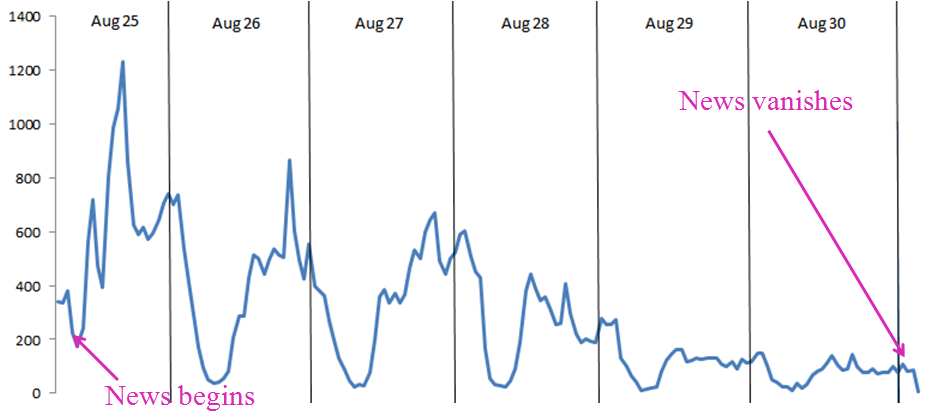
\includegraphics[width=3in,height=1.8in] {pictures/volume1.png}
\label{fig:Volume1}
}
\subfigure[Castro rumor]{
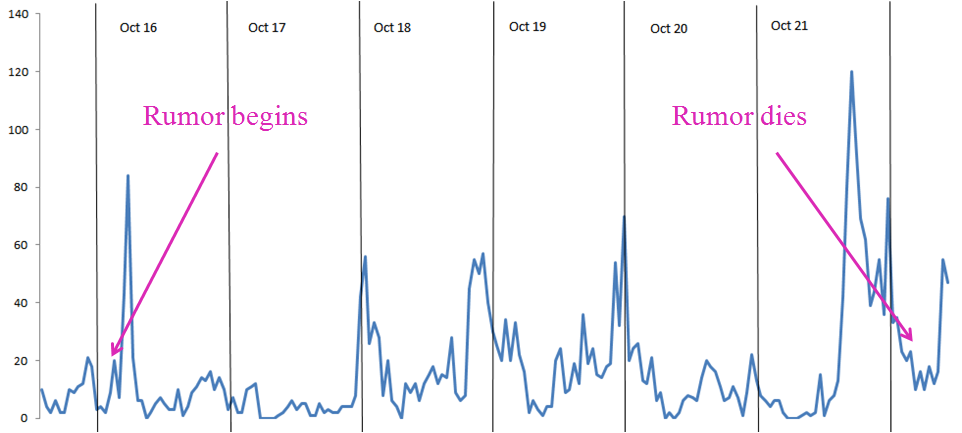
\includegraphics[width=3in,height=1.8in] {pictures/volume2.png}
\label{fig:Volume2}
}
\vspace{-1em}
\caption{Tweet volume.}
\label{fig:Volume}
\end{figure}

\subsection{Rumors}

\noindent
\textbf{\emph{Obama injured.}}
A fake associated press (AP) tweet originated on April 23, 2013 that President
Obama was hurt in White House explosions which caused a brief period of
instability in financial markets. The information was false
and it was determined that the Twitter account was hacked.

\noindent
\textbf{\emph{Doomsday.}}
December 21, 2012 was rumored to be the Doomsday as it marked the end date of a 5126 year long cycle in the Mesoamerican long count calendar. This rumor
spread like wildfire and social networks were flooded with panic and anxiety posts. Considering that we are still alive, Doomsday turned out to
be nothing more than a rumor on a massive scale\footnote{http://en.wikipedia.org/wiki/Doomsday}.

\noindent
\textbf{\emph{Fidel Castro's death.}}
On October 16, 2012 a Naples doctor claimed that former Cuban leader, Fidel Castro suffered a cerebral hemorrhage and is near a
neurovegetative state. However, on October 21, 2012, these rumors were denied
by Elias Jauva, former Venezuelan vice president, who released pictures of him
meeting Castro a few days back\footnote{http://www.inquisitr.com/371007/fidel-castro-allegedly-appears-in-public-after-stroke-rumors/}.

\noindent
\textbf{\emph{Riots and shooting in Mexico.}}
A very interesting example that highlights the perils of rumor spreading on social networks pertains to the false reports of violence and impending attack
in Nezahualcoyotl, %\narenc{Is it the correct spelling? Please checkup carefully. correct}
Mexico. (False) rumors spreading on Twitter and Facebook
about shootouts caused (real) panic and chaos in Mexico City
on September 5, 2012. Interestingly, authorities themselves
turned to Twitter to deny
these rumors\footnote{http://www.foxnews.com/world/2012/09/08/tweets-false-shootouts-cause-panic-in-mexico-city/}.



\begin{figure}[t]
\centering
\subfigure[Amuay explosion]{
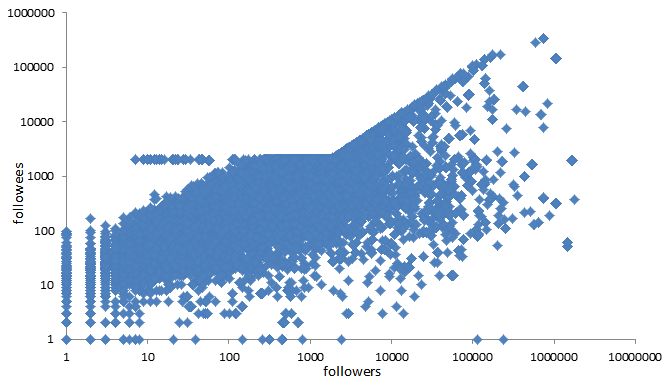
\includegraphics[width=3in,height=1.8in] {pictures/rumor1-scatter.png}
\label{fig:Follow1}
}
\subfigure[Castro rumor]{
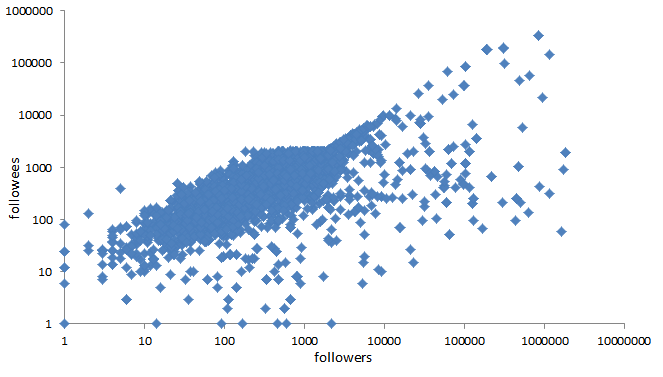
\includegraphics[width=3in,height=1.8in] {pictures/rumor2-scatter.png}
\label{fig:Follow2}
}
\vspace{-1em}
\caption{Followers/followees distributions. Followers: people who follow the person; Followees: people who are followed by the person.}
\label{fig:Followers}
\end{figure}
%\footnote{http://confusedofcalcutta.com/2009/01/11/of-followers-and-followees-and-friends/}

%\subsection{Twitter news collection }
%During data collection from Twitter, our main concern was to obtain pure tweets which are highly related to the news events. We used a customized set of keyword lists and hashtags for filtering the tweets. For each story, we created topic-exclusive keyword list and filtered the relevant tweets by matching the keywords. More story-specific tweets were identified by using a list of $\#$hashtags.
%
%As our stories span across geographic locations and languages, we used several different measures to collect the data. For example, four out of the eight stories are from South America, and hence during data collection for these stories we restricted ourselves to the tweets originating from South America and written either in Spanish or Portuguese. Table 1 list out all the restrictions that were used in collecting the tweets. Further, for each of these topics, we tried to collect the tweets from the beginning of the topic birth to its death. The only exception is the Doomsday rumor for which there is not fixed beginning date. Date range for data collection, along with the keywords, hashtags and tweet counts are mentioned in Table~\ref{table:story-intro} for each of the news story.

\begin{figure*}[t]
\centering
\subfigure[Amuay Cascade]{
   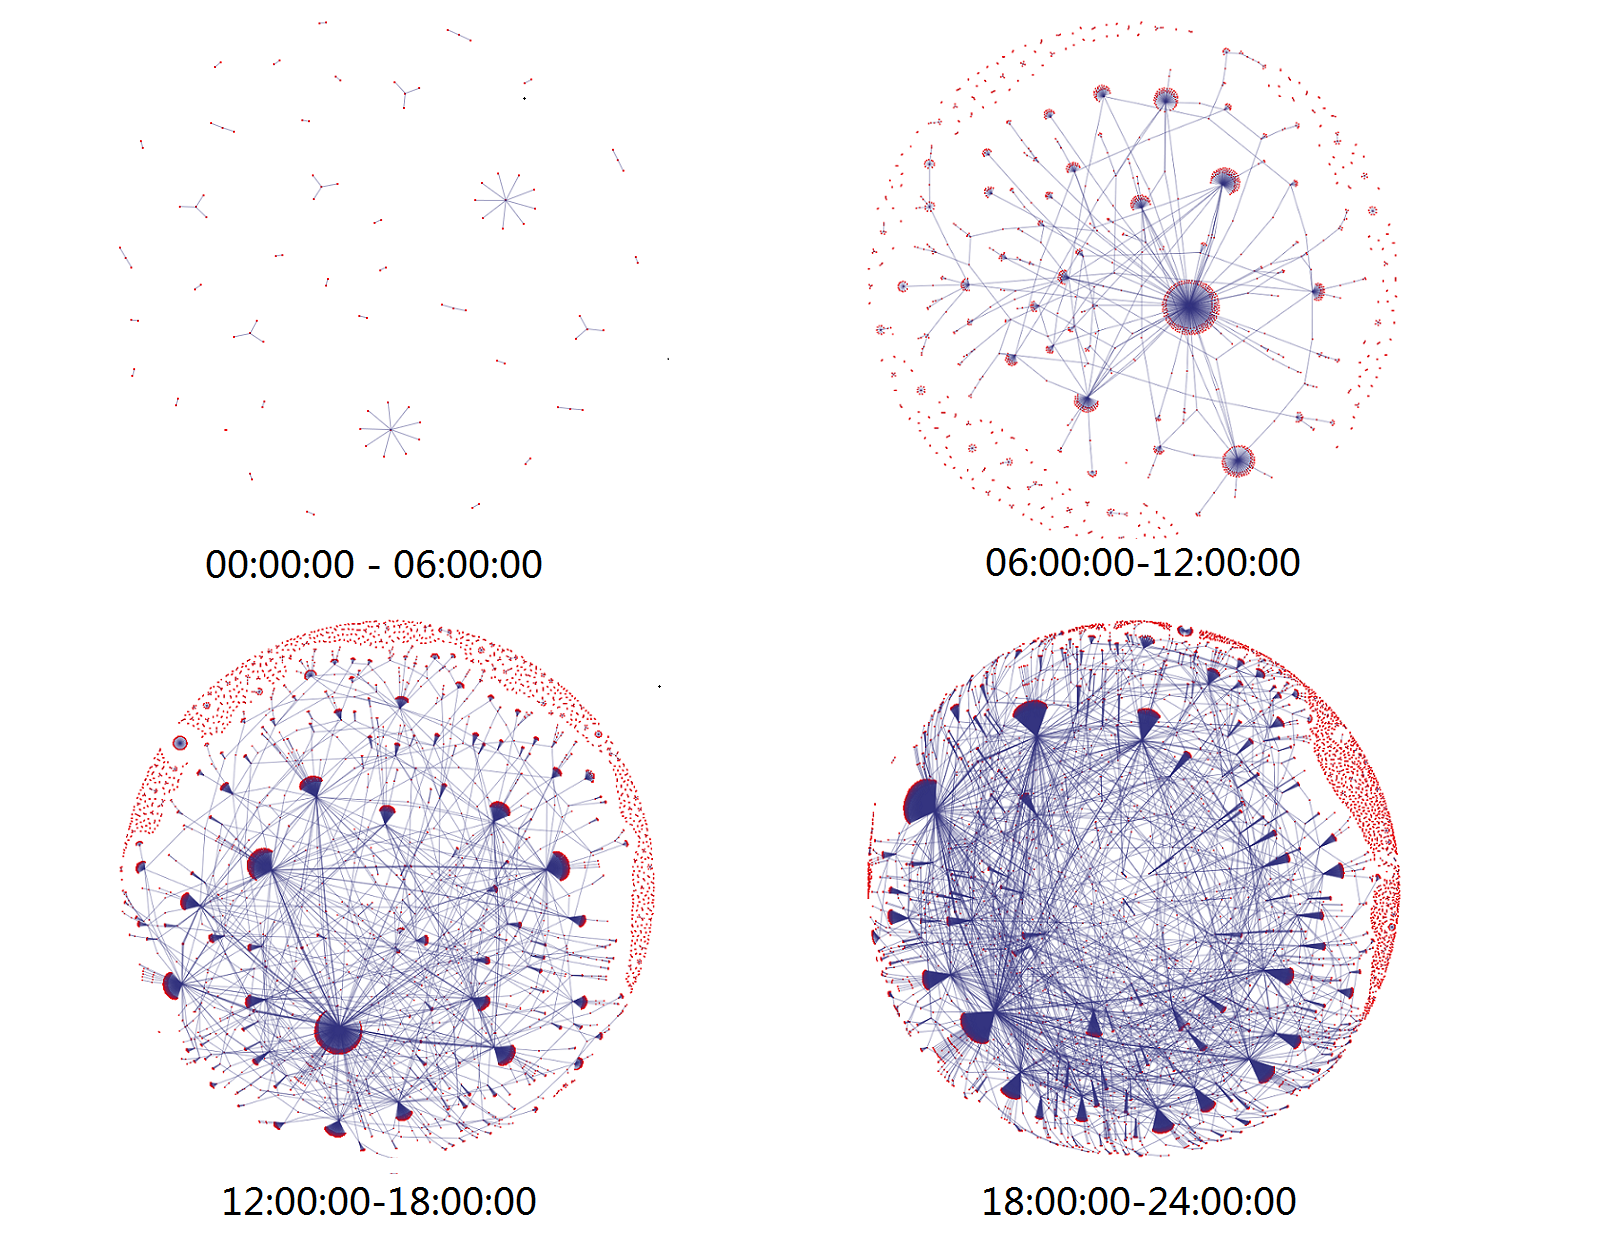
\includegraphics[width=3in,height=2.5in] {pictures/news.png}
   \label{fig:gas-cascade}
 }
  \subfigure[Castro Cascade]{
   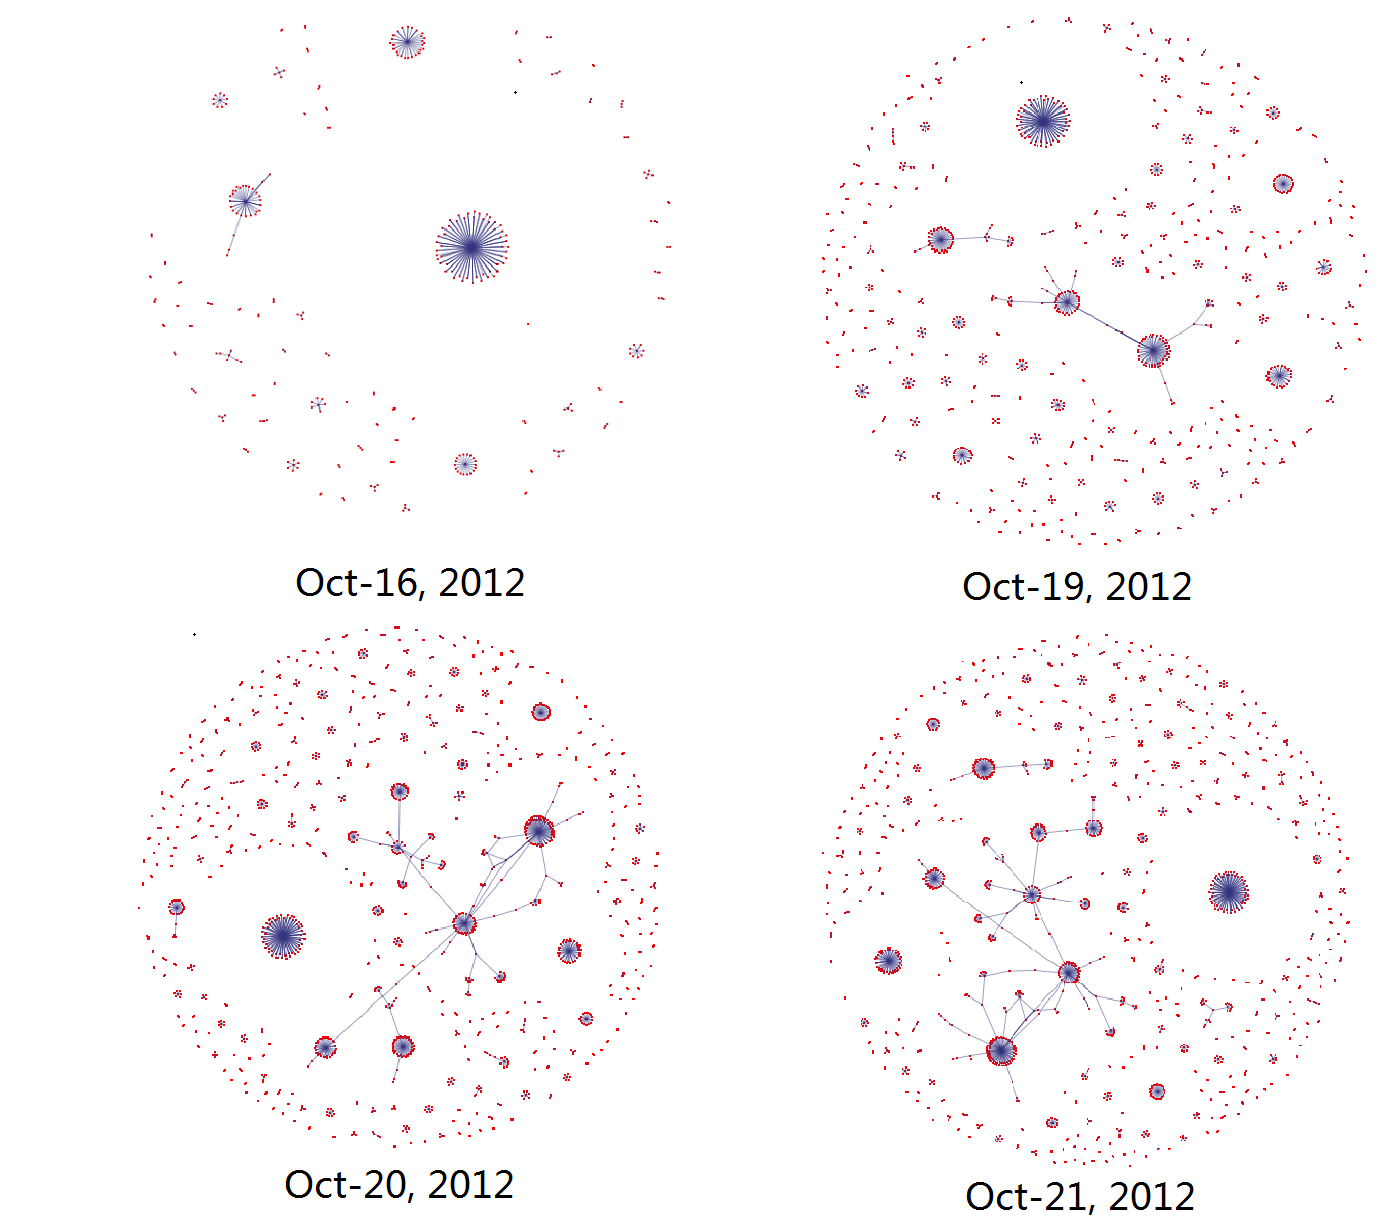
\includegraphics[width=3in,height=2.5in] {pictures/rumor.png}
   \label{fig:Castro-cascade}
 }

\caption{Retweet cascade for the Amuay Explosion news and Castro rumor. Each node is a user id, and each edge connects the retweet user to the original user.}
\label{fig:full-cascade}
\end{figure*}


\subsection{Preliminary Analysis}
We compare the basic properties of news and rumor propagation,
by characterizing
tweet volume over time, follower/followee distributions, the `response ratio'
of a story, and the retweet cascades. In order to maintain brevity, we show
results from only two stories in this section: one from our news
collection (the Amuay explosion) and one from our rumor collection (Fidel
Castro's purported death).

\textbf{Tweet Volume.} For both examples, we plot the tweet volume over time from the beginning of the story. Figure~\ref{fig:Volume1} shows the activity for the
2012 Amuay refinery explosion example. An activity burst was formed immediately after the news was made public. The number of tweets dropped progressively as the days went by. This activity trend displays attributes similar to breaking news propagation as described by Mendoza
et al.~\cite{Mendoza:2010}. In contrast, Figure~\ref{fig:Volume2} depicts
the volume of tweets about a rumor regarding the health of the
former Cuban leader Fidel Castro. Here we see
occasional spikes of
tweet volume; note the increase in tweet volume
around October 21st, when the rumors were officially denied.

\textbf{Followers and Followees Distributions.} Figure~\ref{fig:Follow1} is a log-log
scatter plot of the followers/followees distribution about
the Amuay explosion news, and Figure~\ref{fig:Follow2} is the corresponding
plot about Fidel Castro's death rumor. There is no significant
qualitative or quantitative difference in this case; in particular both
plots show that
the number of followees is less than the number of followers.
%Table~\ref{table:follower} gives the details: %in Amuay dataset, 33936 users
%%register more followers than followees (69\%),
%%14936 users register more followees than followers, and 143 users register
%%the same number of followers and followees.
%Amuay news and the Fidel Castro rumor exhibits comparable percentages for follower and followee.

%\begin{table}[ht]
%\centering
%\caption{Follower (ER) and followee (EE) distribution for two datasets.}
%\label{table:follower}
%\begin{tabular}{|c|c|c|l|} \hline
%&ER>EE&ER=EE&ER<EE\\ \hline
%Amuay news & 33936 (69\%)& 143 (1\%)&14936 (30\%)\\
%Castro rumor &2549 (66\%)& 13 (0.4\%)&1073 (33\%)\\ \hline
%\end{tabular}
%\end{table}

\textbf{Response Ratio.} A tweet can either be a post made by the
user's initiative,
or a responsive post  to some other user's post (e.g., retweets and replies).
As Starbird et al.~\cite{Starbird:2012} discuss, retweets reveal how
information propagates through a social network: the `deeper' a retweet, the
more relevant the tweet is for the community. Based on this idea,
we define the response ratio of a story as the fraction of responsive tweets
to the total number of tweets in the story.
Table~\ref{table:story-intro} lists the response ratio for all the 8 stories. As we can see, response ratios for news are higher than that for the rumors.
%\narenc{You keep using different names: response ratio, responsiveness ratio,
%response rate, responsiveness rate. Pick one and stick with it.
%Lets use response ratio because I don't think you are computing any `rate'.}
%\narenc{You have now removed that column from the table. Put it back.}

\textbf{Retweet Cascades.} A retweet cascade reflects how the social media network propagates information. Figure~\ref{fig:full-cascade} depicts the evolution of the retweet graphs for the Amuay news and Castro rumor dataset. For Amuay news, we plot four graphs with intervals of 6 hours,
% to show the dynamic process of the information flow on the Twitter.
depicting that a burst has been formed during 6am-12am, only 5 hours after the accident.
 %In the following hours, ten of thousands of users got this news from many sources.
 Fig.~\ref{fig:Castro-cascade} shows the retweet graphs of the rumor for several days. We can see
% that there are several central information sources to expand the rumor on Oct 16th, 2012.
 even after one day, there is no burst of tweets related to this rumor.
% After the clarification of the rumor, a little more users are involved in the re-tweet network.
 Compared with the network between the news and rumors, we find several features about the rumor.
% 1) In the initial  stage of the rumor, several central information sources posts the rumors.
1) The network for the news instance
is more complex and users can obtain news from many sources, while users obtain
the rumor information only from limited information centers. 2) There is an immediate burst after a news is made public while there is no obvious burst for the rumors.

%\narenc{What do people learn from this paragraph and the picture? Can you plot
%it for the Castro rumor? Does it look different?}

%\textbf{Can we learn more?} Although these properties provide us
%with some discriminating information, they still do not help
%develop a model-based approach for how news propagates differently
%from rumors, which is our focus next.

%with good amount of information we still can't quantify how news propagates over time. Also it would be interesting to know how information cascades were generated in a step by step manner over space. Hence, in this chapter, we propose a diffusion method and an event-driven model to find answers to the above mentioned problems. We represent Twitter network as a graph with vectors and edges and apply two epidemic models to simulate how vectors and edges grow with time. More specifically, we propose a 1-step graph transition method to simulate the graph growing process. By monitoring the step by step propagation process, we quantify transfer deviation using our event-driven model.

\section{Our Approach}
As stated earlier, we used compartmental population models to quantify the propagation of news and rumors on Twitter, focusing primarily on the SIS and SEIZ models.

\subsection{SIS}
As described earlier, this model divides the population into two compartments, or classes: susceptible and infected.
Note that in this model, infected individuals return to the susceptible class on recovery because the disease confers no immunity against reinfection.


In order to adapt this model for Twitter, we have given new meaning to these terms. An individual is identified as infected (I) if he posts a tweet about the topic of interest, and susceptible (S) if he has not. A consequence of this interpretation is that an individual posting a tweet is retained to the infected compartment indefinitely; hence, he can not propagate back to the susceptible class as is possible in an epidemiological application. At any given time period $t$, we use $N(t)$ to denote the total population size, $S(t)$ the susceptible population size, and $I(t)$ the infected population size, such that $N(t) = I(t) + S(t)$. As shown in Figure~\ref{fig:sis-framework}, the SIS spreading rule can be summarized as follows:

\begin{figure}[ht]
\centering
%\epsfig{file=word.pdf, width=3in}
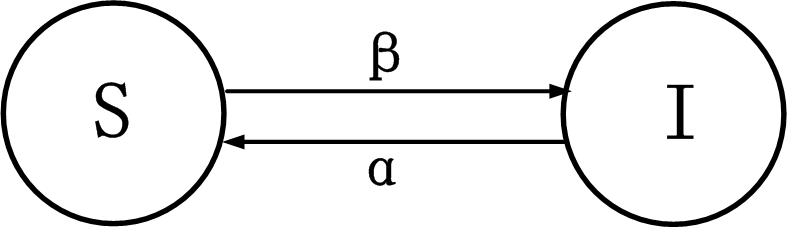
\includegraphics[width=2.5in]{pictures/SIS.png} %?????????????
\vspace{-1em}
\caption{SIS model framework}
\label{fig:sis-framework}
\end{figure}


\begin{figure}[ht]
\centering
%\epsfig{file=word.pdf, width=3in}
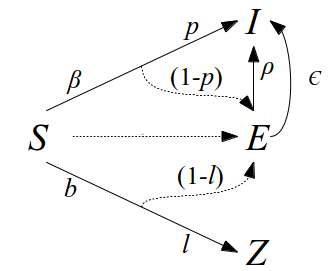
\includegraphics[width=2.5in]{pictures/SEIZ.png} %?????????????
\vspace{-1em}
\caption{SEIZ model framework}
\label{fig:seiz-framework}
\end{figure}


\begin{itemize}
\item An individual that tweets about a topic is regarded as infected.
\item A susceptible person has not tweeted about the topic.
\item A susceptible person coming into contact with an infected individual (via a tweet) becomes infected himself, thus immediately posting a tweet.
\item Susceptible individuals remain so until coming into contact with an infected person.
\end{itemize}

\begin{figure}[t]
\centering
  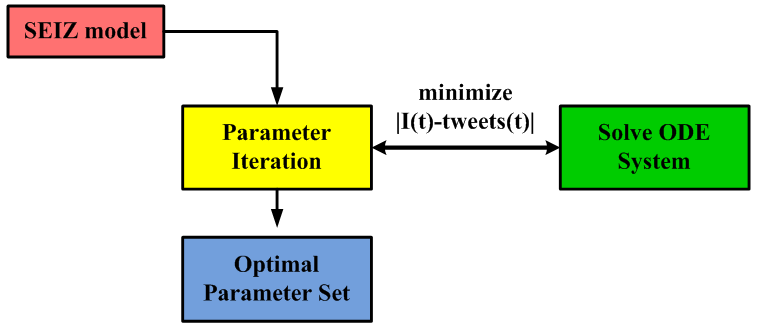
\includegraphics[width=3in]{pictures/implementation_flow.png}
  \vspace{-1em}
  \caption{Numerical implementation work-flow.
 % For both the SIS and SEIZ models, a nonlinear least squares fit of each ODE system to Twitter data identifies an optimal parameter set by minimizing the difference between the Infected compartment and the Twitter data.
  }
  \label{fig:implementation_flow}
\end{figure}

\noindent
The SIS model is mathematically represented by the following system of ordinary differential equations (ODEs)~\cite{murray2002mathematical}:

\begin{subequations}\label{eq:sis}
\begin{align}
&\frac{d [S]}{dt} = -\beta S I + \alpha I \\
&\frac{d [I]}{dt} = \beta S I - \alpha I
\end{align}
\end{subequations}


\subsection{SEIZ}
One drawback of the SIS model is that once a susceptible individual gets exposed to disease, he can only directly transition to infected status. In fact, especially on Twitter, this assumption does not work well; people's ideologies are complex and when they are exposed to news or rumors, they may hold different views, take time to adopt an idea, or even be skeptical to some facts. In this situation, they might be persuaded to propagate a story, or commence only after careful consideration themselves. Additionally, it is quite conceivable that an individual can be exposed to a story (i.e. received a tweet), yet never post a tweet themselves.

Based on this reasoning, we considered a more applicable, robust model, the SEIZ model which was first used to study the adoption of Feynman diagrams~\cite{powerofgoodidea:2006}. In the context of Twitter, the different compartments of the SEIZ model can be viewed as follows: Susceptible (S) represents a user who has not heard about the news yet; infected (I) denotes a user who has tweeted about the news; skeptic (Z) is a user who has heard about the news but chooses not to tweet about it; and exposed (E) represents a user who has received the news via a tweet but has taken some time, an exposure delay, prior to posting. We note that referring to the Z compartment as skeptics is in no way an implication of belief or skepticism of a news story or rumor. We adopt this terminology as this was the nomenclature used by the original authors of the SEIZ model~\cite{powerofgoodidea:2006}.

A major improvement of the SEIZ model over the SIS model is the incorporation of exposure delay. That is, an individual may be exposed to a story, but not instantaneously tweet about it. After a period of time, he may believe it and then be promoted to the infected compartment. Further, it is now possible for an individual in this model to receive a tweet, and not tweet about it themselves. As shown in Figure~\ref{fig:seiz-framework}, SEIZ rules can be summarized as follows:

\begin{table}[t] %!htp
\small
\caption{Parameter definitions in SEIZ model\cite{powerofgoodidea:2006}}
\vspace{0.5em}
\centering
\begin{tabular}{ p{4cm}  p{8cm} }
\hline
\textbf{Parameter} & \textbf{Definition} \\ [1ex]
\hline
$\beta$ & S-I contact rate \\[1ex]
b & S-Z contact rate \\[1ex]
$\rho$ & E-I contact rate \\[1ex]
$\epsilon$ & Incubation rate \\[1ex]
1/$\epsilon$ &  Average Incubation Time \\[1ex]
bl & Effective rate of S -\textgreater Z  \\ [1ex]
$\beta\rho$ & Effective rate of S -\textgreater I  \\ [1ex]
b(1-l) & Effective rate of S -\textgreater E via contact with Z  \\ [1ex]
$\beta (1-p)$ & Effective rate of S -\textgreater E via contact with I \\ [1ex]
l & S-\textgreater Z Probability given contact with skeptics \\[1ex]
1-l & S-\textgreater E Probability given contact with skeptics \\ [1ex]
p & S-\textgreater I Probability given contact with adopters \\ [1ex]
1-p & S-\textgreater E Probability given contact with adopters \\ [1ex]
\hline
\end{tabular}
\label{table:parameters}
\end{table}



\begin{itemize}
\item Skeptics recruit from the susceptible compartment with rate $b$, but these actions may result either in turning the individual into another skeptic
(with probability $l$), or it may have the unintended consequence of sending that person into the exposed (E) compartment with probability $(1 - l)$.
\item A susceptible individual will immediately believe a news story or rumor with probability $p$, or that person will move to the exposed (E) compartment with probability $(1 - p)$.
\item Transitioning of individuals from the exposed compartment to the infected class can be caused by one of two separate mechanisms: (i) an individual in the exposed class has further contact with an infected individual (with contact rate $\rho$), and this additional contact promotes him to infected; (ii) an individual in the exposed class may become infected purely by self-adoption (with rate $\epsilon$), and not from additional contact with those already infected. \end{itemize}


The SEIZ model is mathematically represented by the following system of ODEs. A slight difference of our implementation of this model is that we do not incorporate vital dynamics, which includes the rate at which individuals enter and leave the population $N$ (represented by $\mu$~\cite{powerofgoodidea:2006}). In epidemiological disease applications, this encompasses the rate at which people become susceptible (e.g. born) and deceased. In our application, a Twitter topic has a net duration not exceeding several days. Thus, the net entrance and exodus of Twitter users over these relatively short time periods is not expected to noticeably impact compartment sizes and our ultimate findings\footnote{http://www.statisticbrain.com/twitter-statistics/}.

\begin{subequations}\label{eq:seiz}
\begin{align}
\frac{d [S]}{dt} &= -\beta S \frac{I}{N} - bS \frac{Z}{N} \\
\frac{d [E]}{dt} &= (1-p)\beta S\frac{I}{N} + (1-l)bS\frac{Z}{N}-\rho E\frac{I}{N} -\epsilon E \\
\frac{d [I]}{dt} &= p\beta S \frac{I}{N} + \rho E \frac{I}{N} + \epsilon E \\
\frac{d [Z]}{dt} &= lbS \frac{Z}{N}
\end{align}
\end{subequations}


\subsection{Practical Issues}
During our adoption of the SIS and SEIZ models to understand Twitter datasets, we were constrained by several factors. The first constraint was the unknowns in the models. For example, we do not know the transition rates between the compartments nor the initial sizes of the compartments.
%The only data available is the Twitter data itself, which we used to leverage information about the infected compartment.


\begin{figure}[t]
\centering
\subfigure[SIS]{
   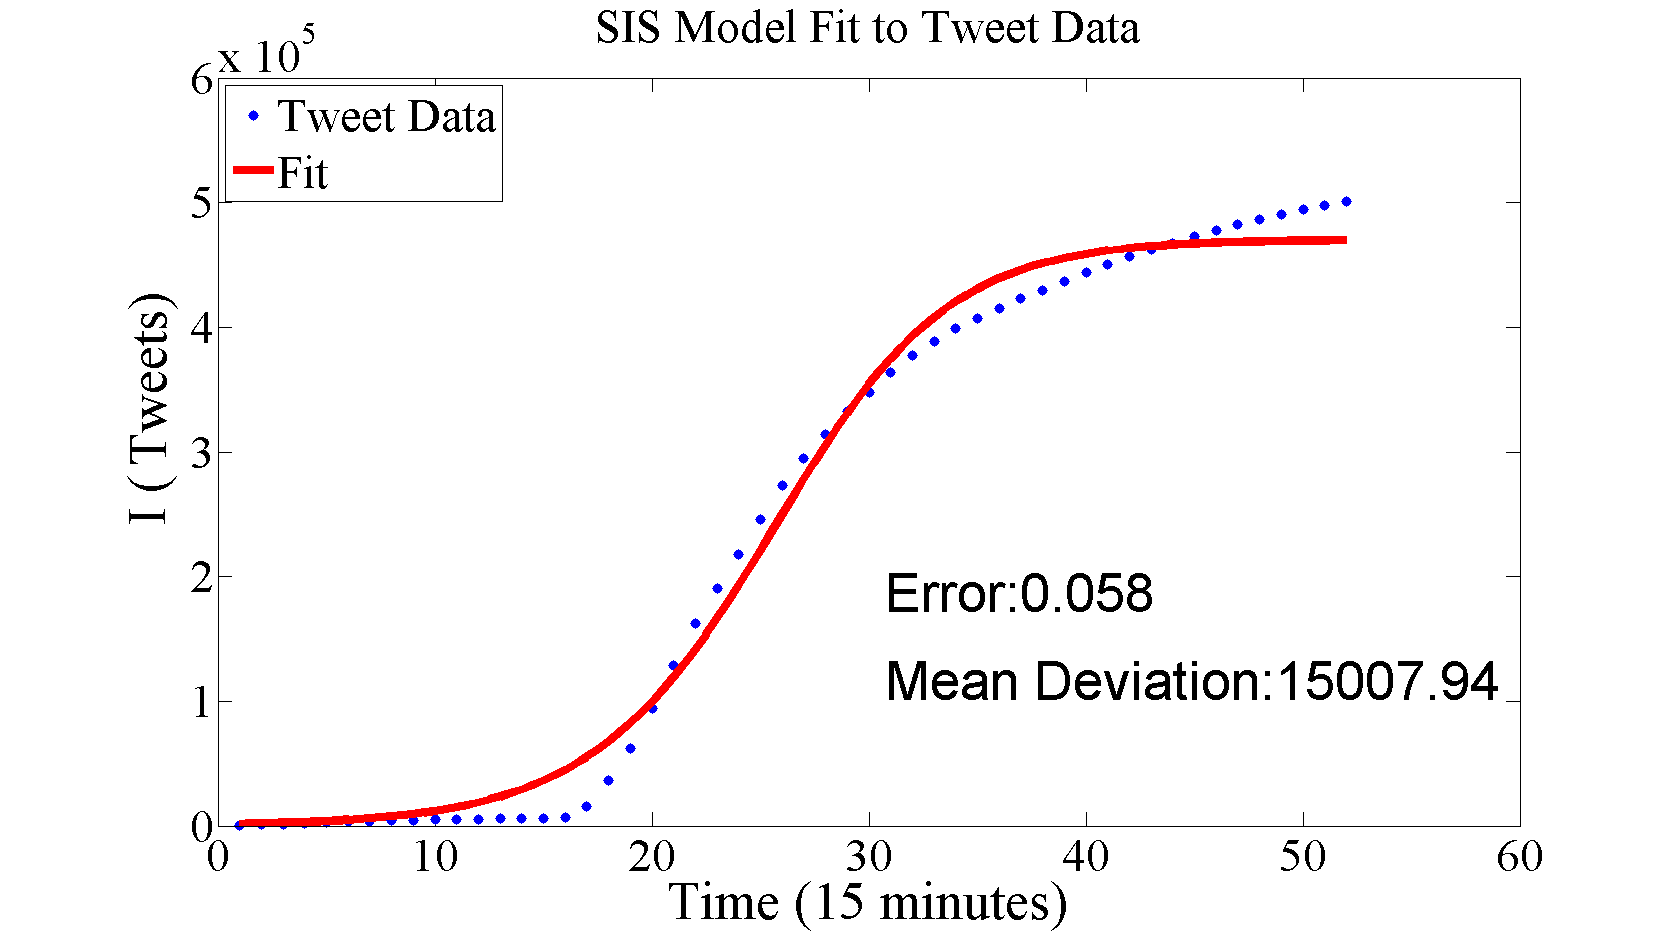
\includegraphics[width=2in,height=1.5in] {pictures/Boston_SIS.png}
  \label{fig:Boston_bombing_sis}
 }
 \subfigure[SEIZ]{
   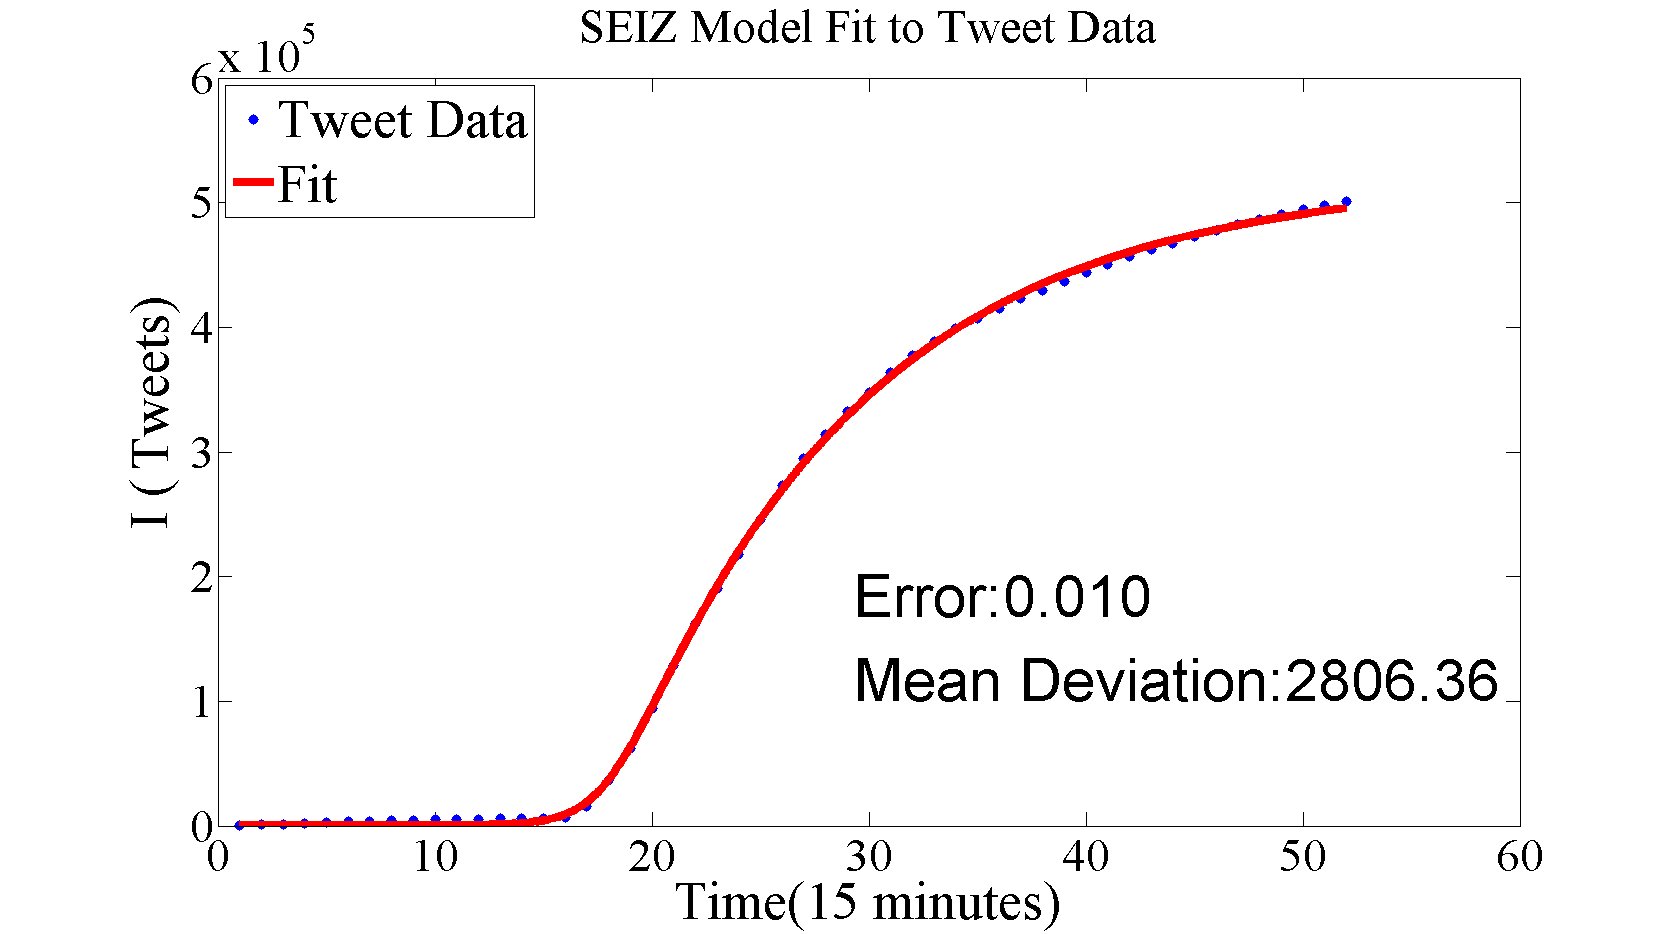
\includegraphics[width=2in,height=1.5in] {pictures/Boston_SEIZ.png}
  \label{fig:Boston_bombing_seiz}
 }
\vspace{-1em}
\caption{Best fit modeling for Boston news.}
\label{fig:Boston_bombing}
\end{figure}


\begin{figure}[t]
\centering
\subfigure[SIS]{
   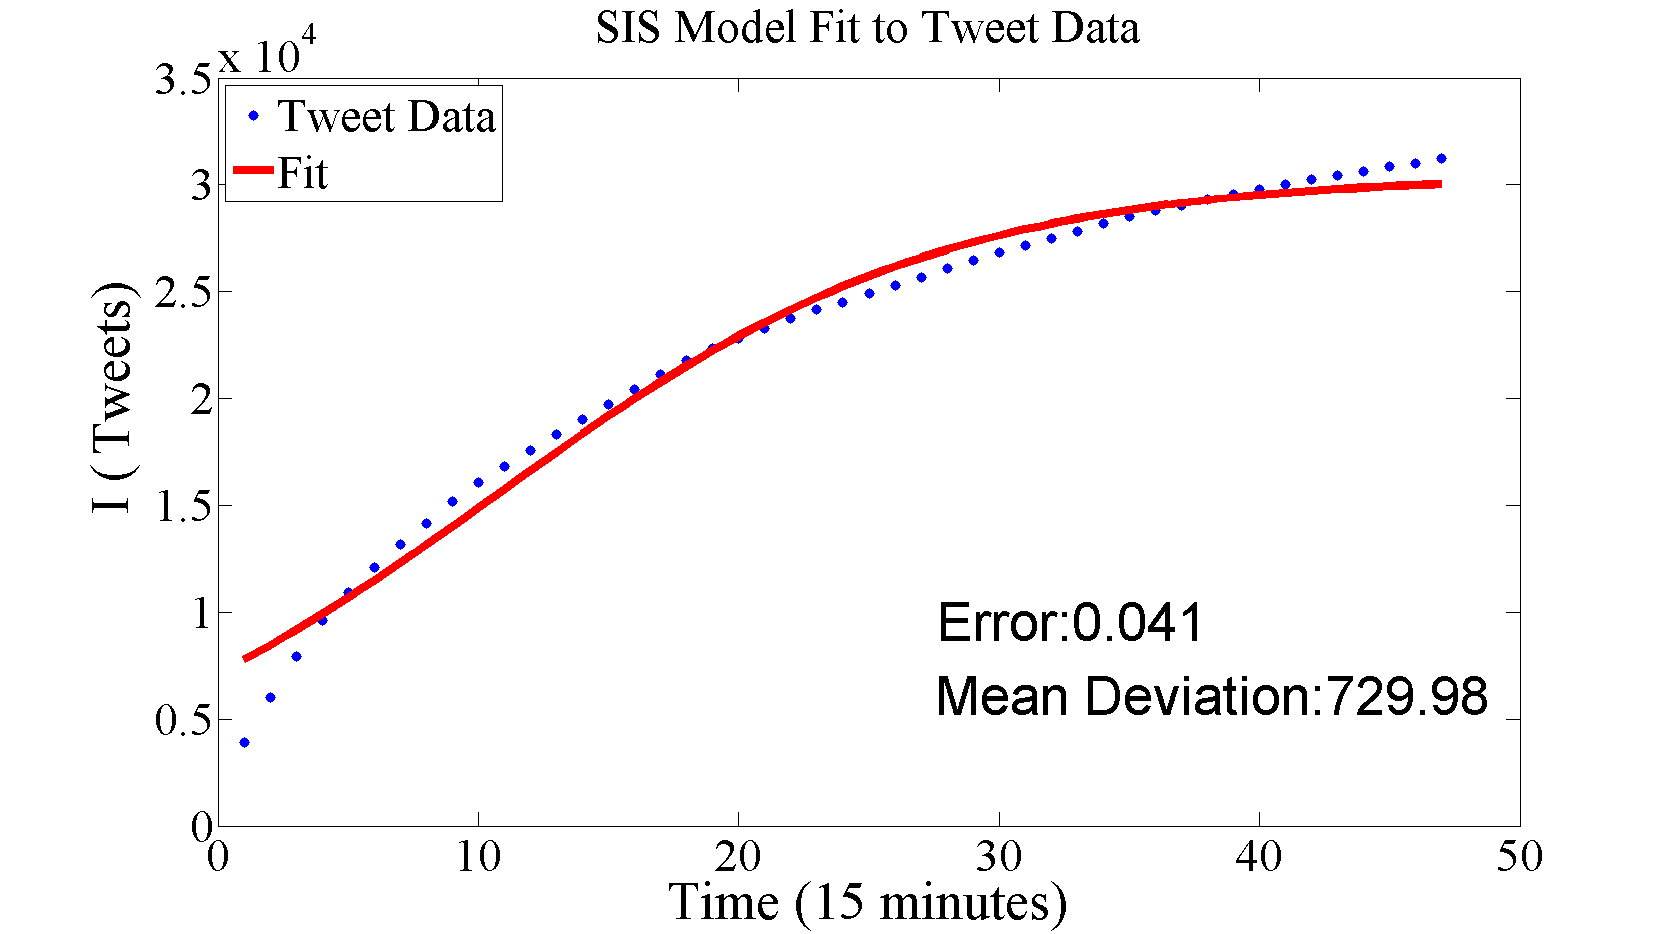
\includegraphics[width=2in,height=1.5in] {pictures/Pope_SIS.png}
  \label{fig:Benedict_sis}
 }
  \subfigure[SEIZ]{
   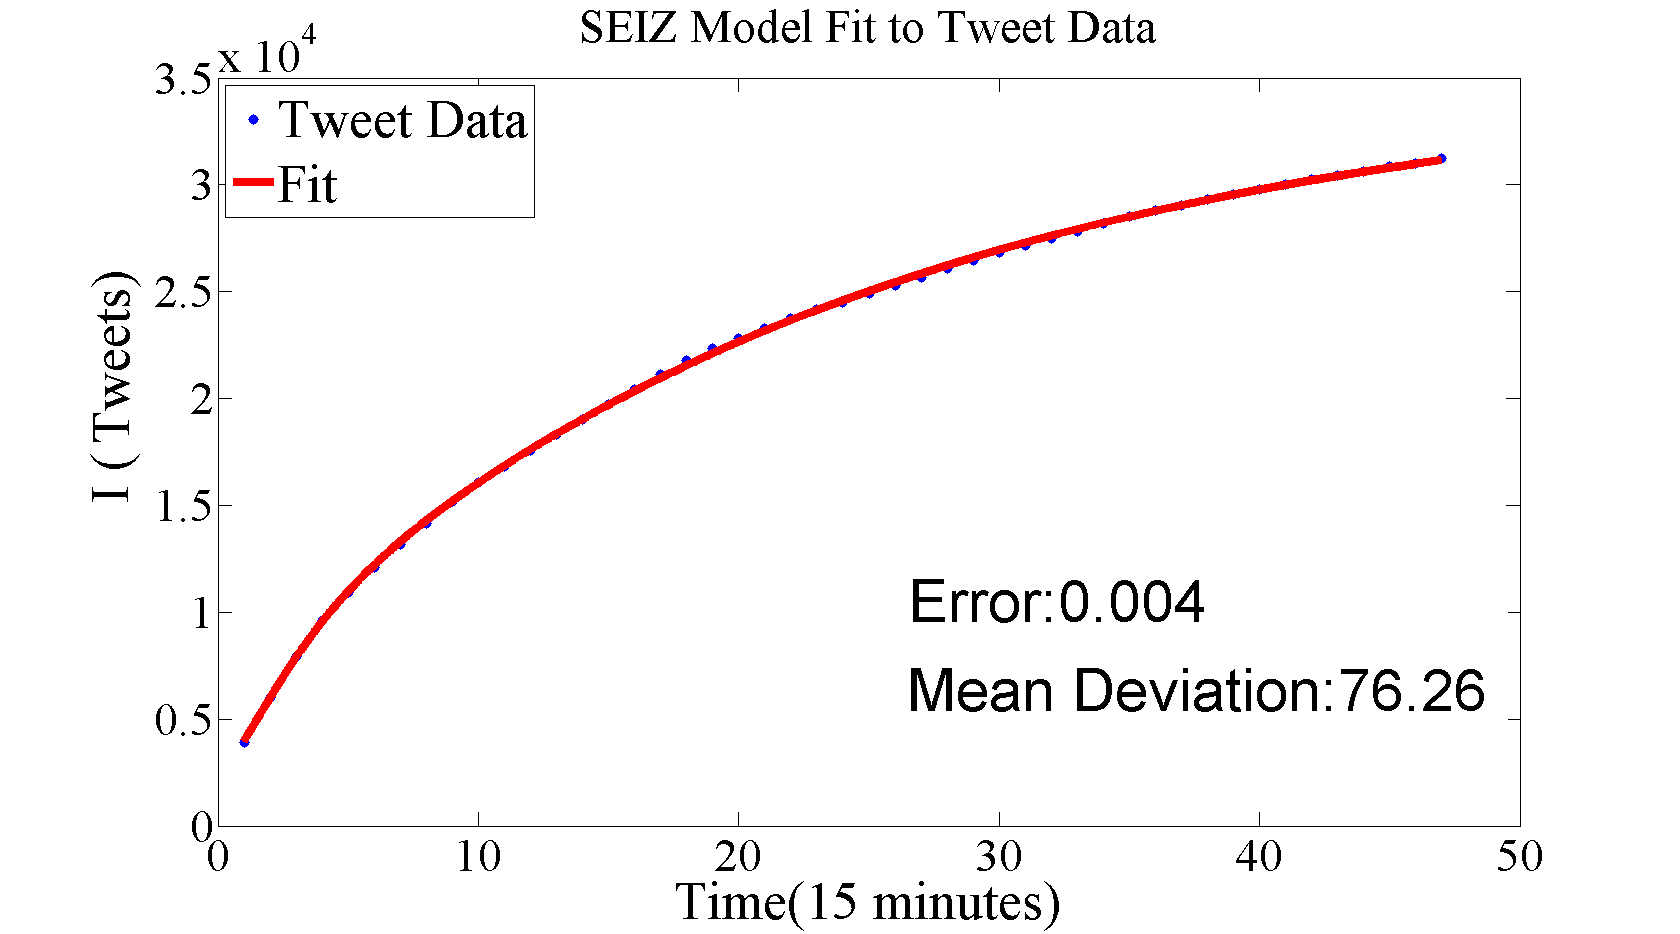
\includegraphics[width=2in,height=1.5in] {pictures/Pope_SEIZ.png}
  \label{fig:Benedict_seiz}
 }
\vspace{-1em}
\caption{Best fit modeling for Pope news.
\label{fig:Benedict}
}
\end{figure}


\begin{figure}[t]
\centering
\subfigure[SIS]{
   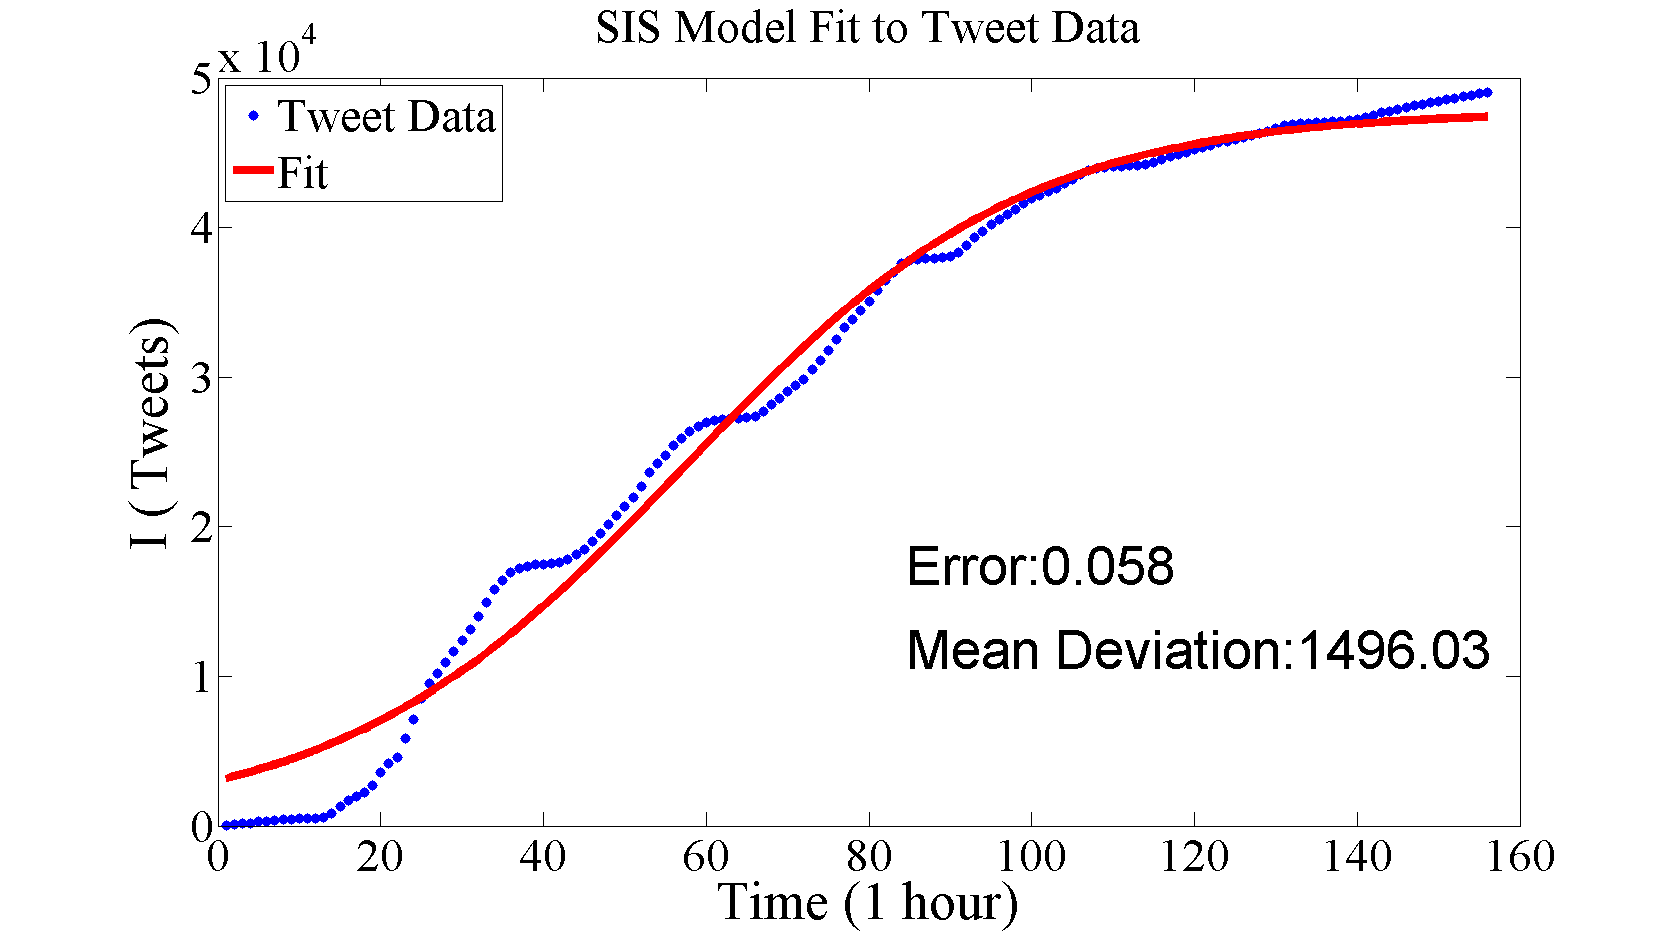
\includegraphics[width=2in,height=1.5in] {pictures/Amuay_SIS.png}
  \label{fig:Gas_explosion_sis}
 }
  \subfigure[SEIZ]{
   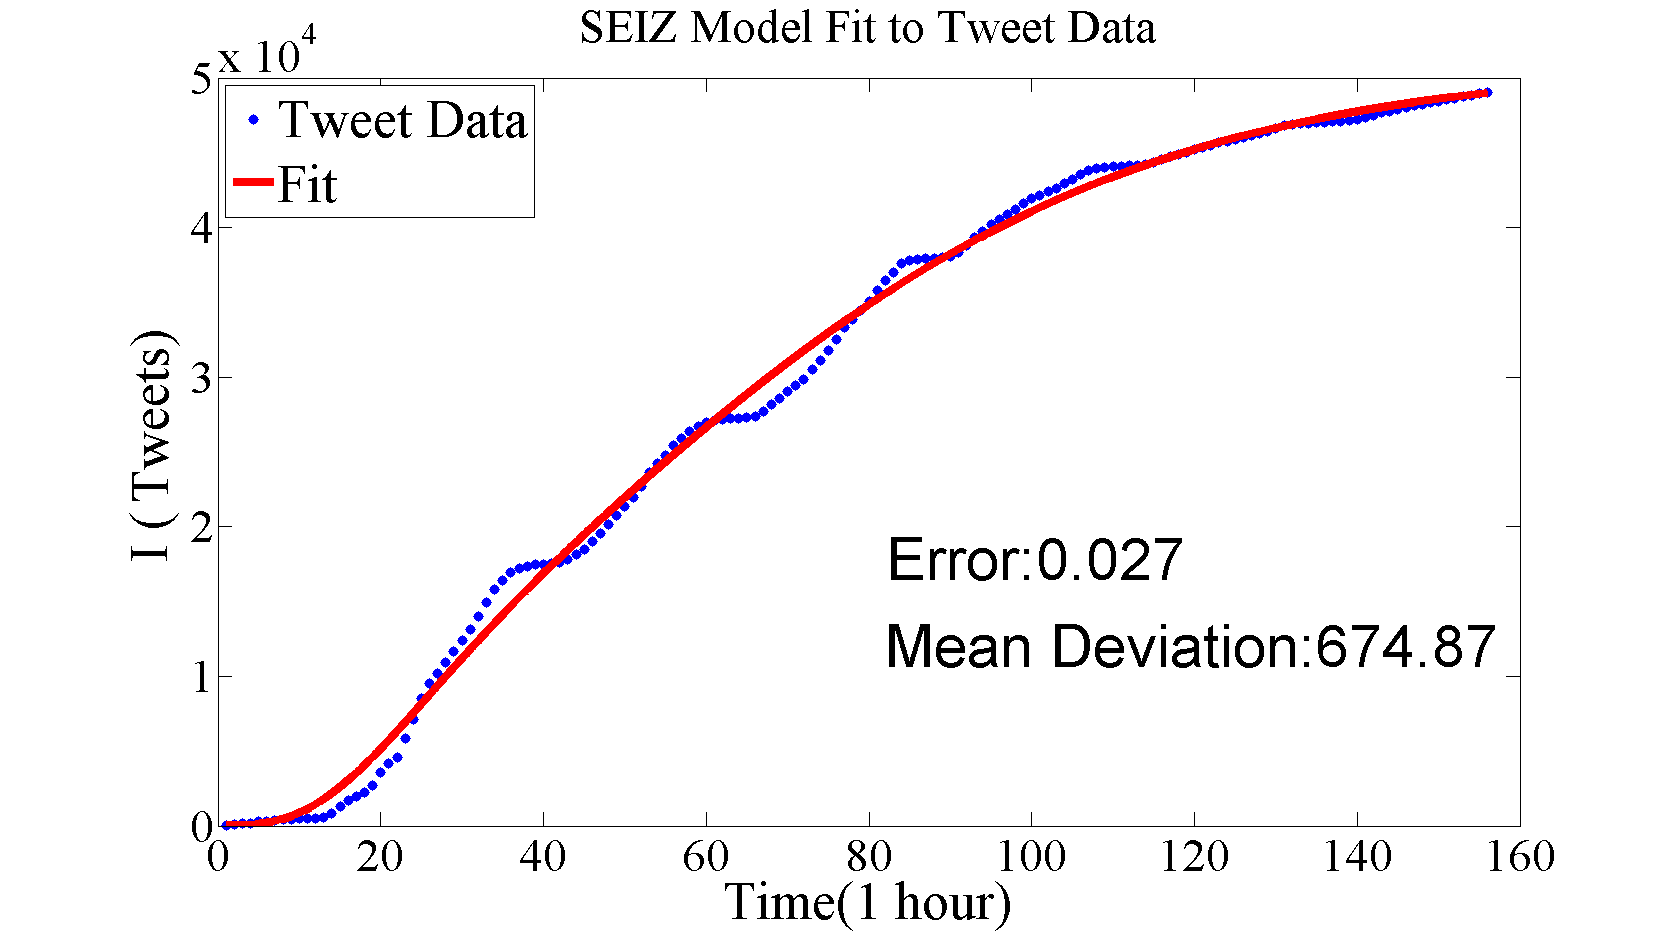
\includegraphics[width=2in,height=1.5in] {pictures/Amuay_SEIZ.png}
  \label{fig:Gas_explosion_seiz}
 }
\vspace{-1em}
\caption{Best fit modeling for Amuay news.}
\label{fig:Gas_explosion}
\end{figure}



\begin{figure}[t]
\centering
\subfigure[SIS]{
   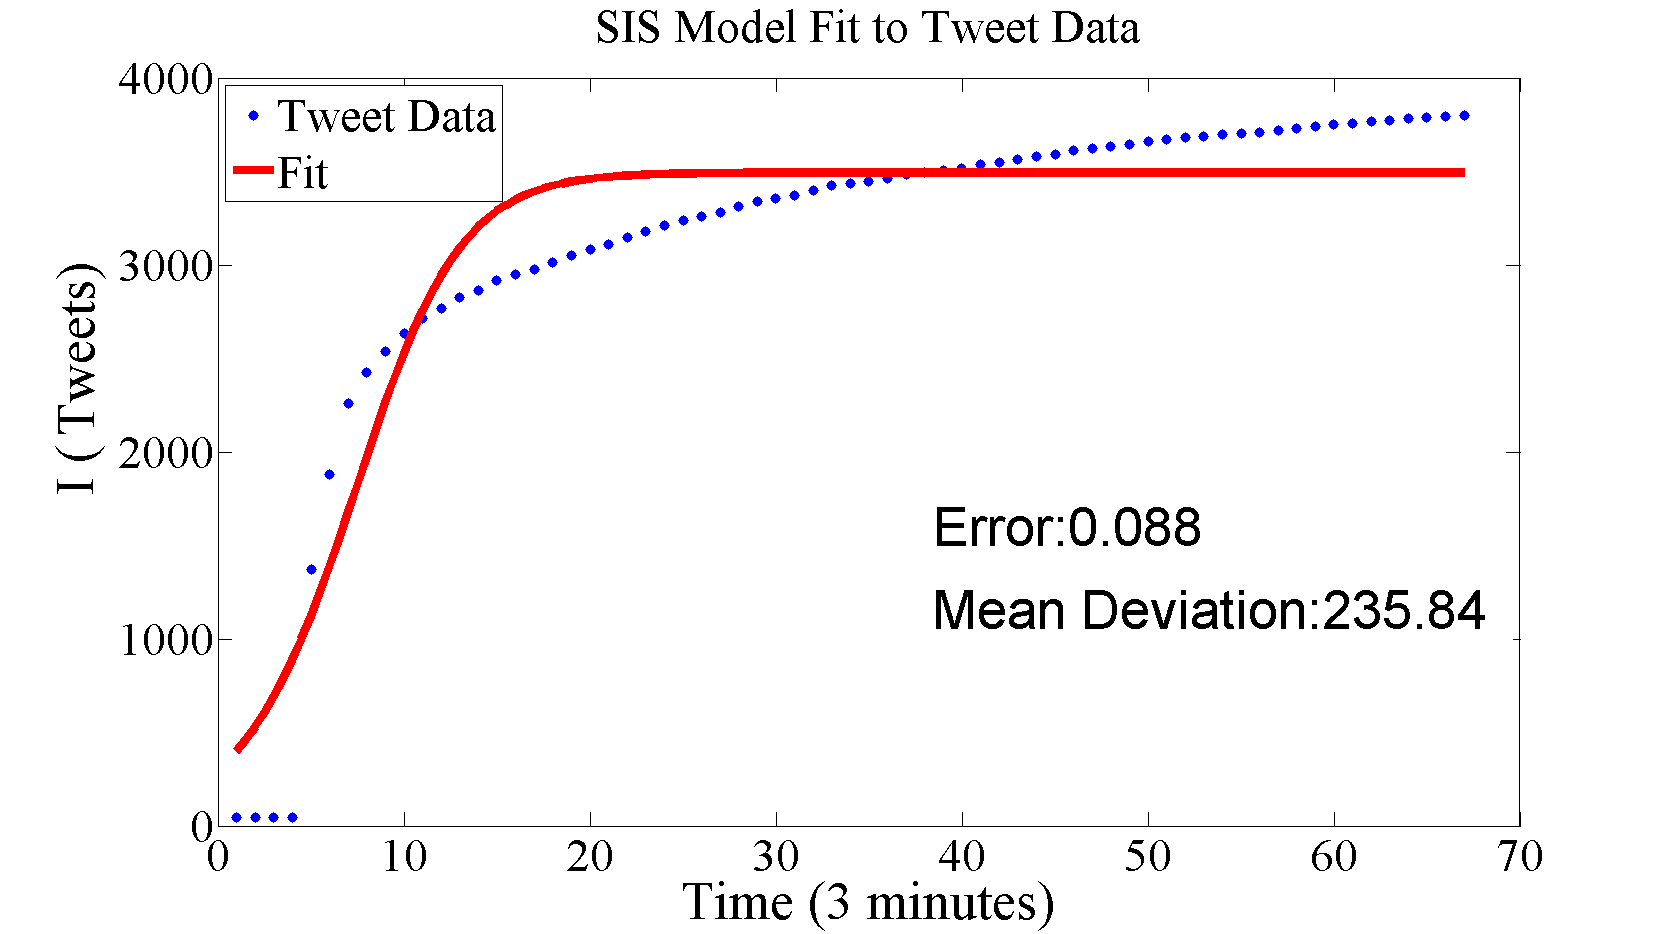
\includegraphics[width=2in,height=1.5in] {pictures/Michelle_SIS.png}
  \label{fig:Michelle_sis}
 }
  \subfigure[SEIZ]{
   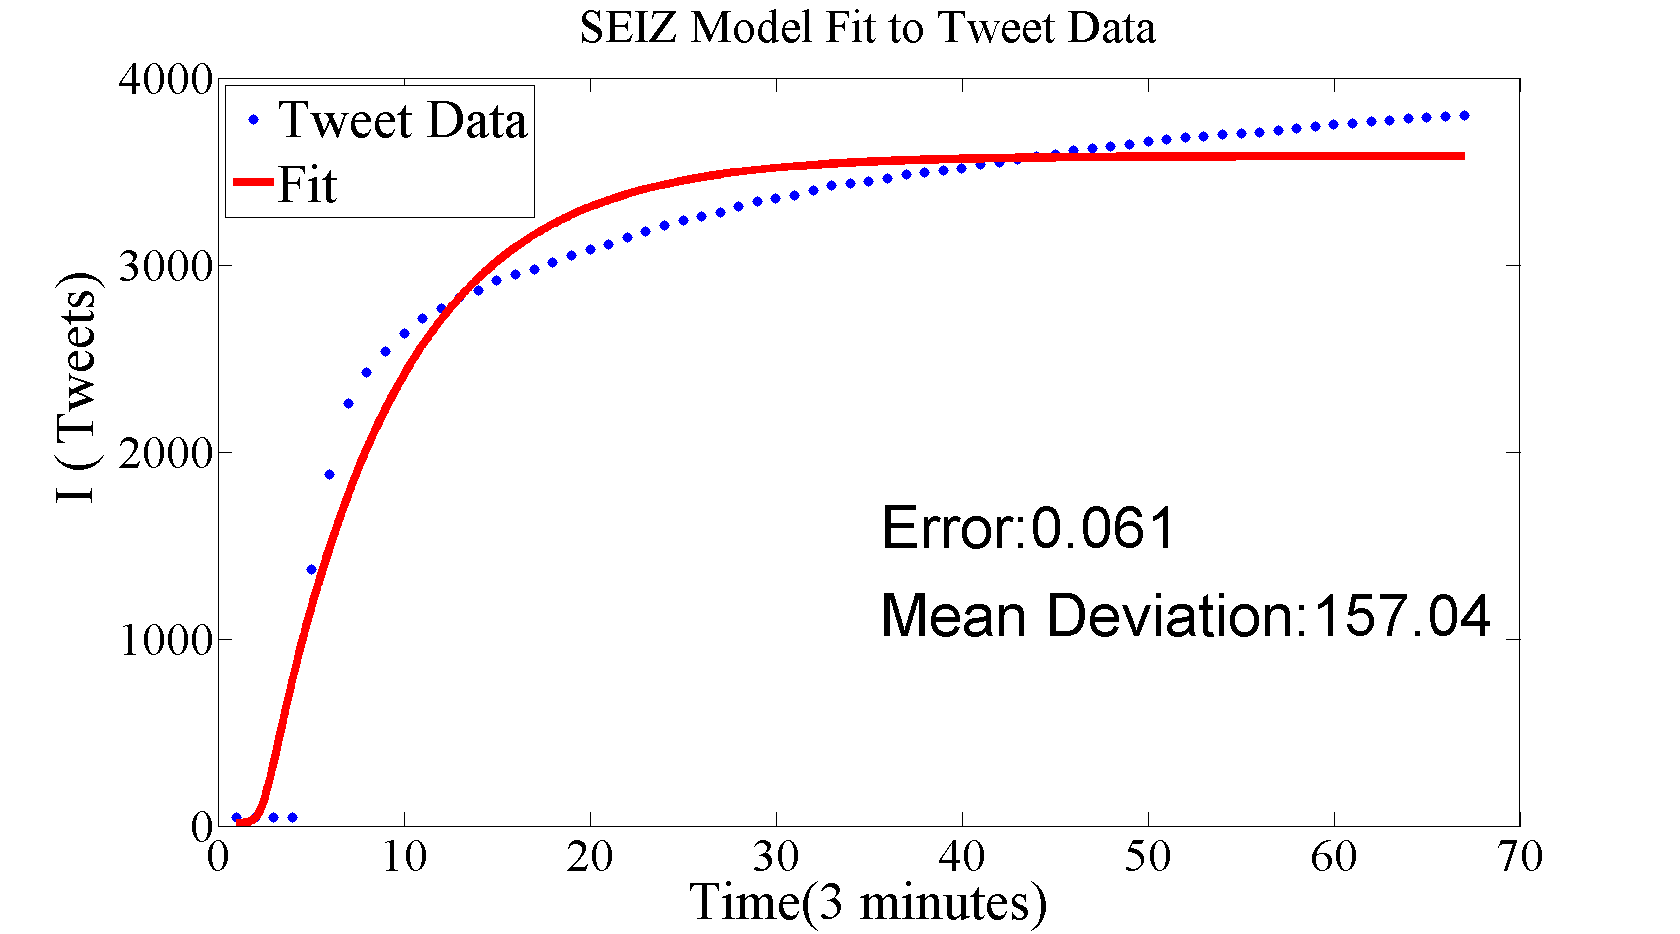
\includegraphics[width=2in,height=1.5in] {pictures/Michelle_SEIZ.png}
  \label{fig:Michelle_seiz}
 }
\vspace{-1.08em}
\caption{Best fit modeling for Michelle news.}
\label{fig:Michelle}
\end{figure}


\begin{figure}[ht]
\centering
\subfigure[SIS]{
   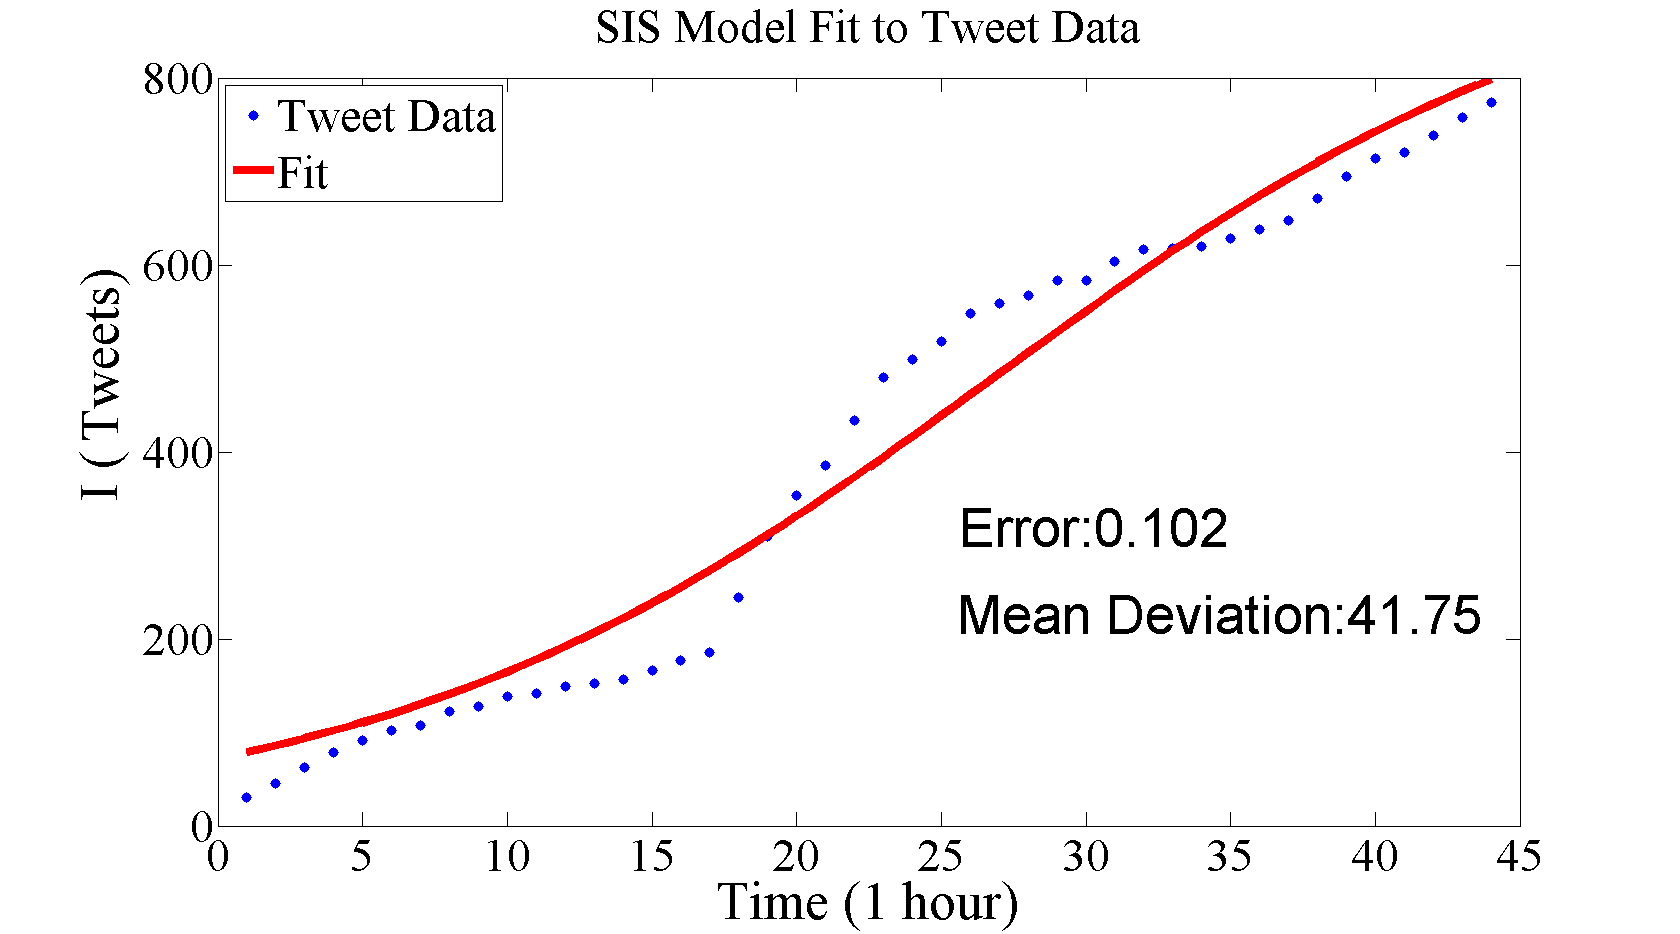
\includegraphics[width=2in,height=1.5in] {pictures/Obama_SIS.png}
  \label{fig:Obama_sis}
 }
 \subfigure[SEIZ]{
   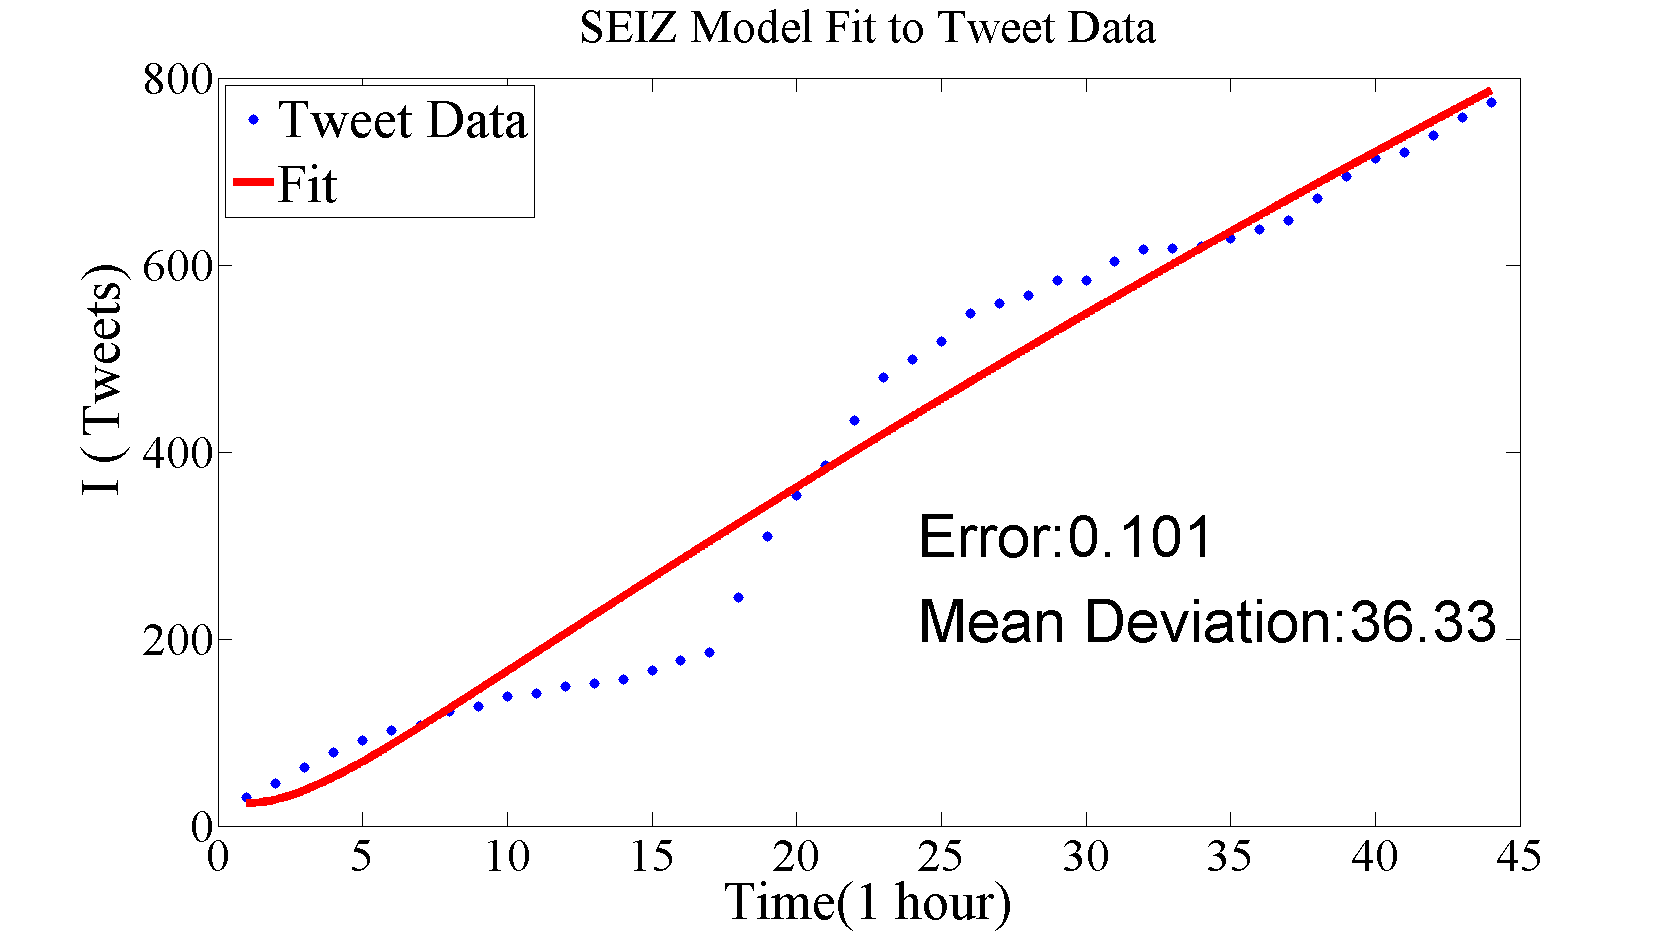
\includegraphics[width=2in,height=1.5in] {pictures/Obama_SEIZ.png}
   \label{fig:Obama_seiz}
 }
\vspace{-1em}
\caption{Best fit modeling for Obama news.}
\label{fig:Obama}
\end{figure}


\begin{figure}[ht]
\centering
\subfigure[SIS]{
   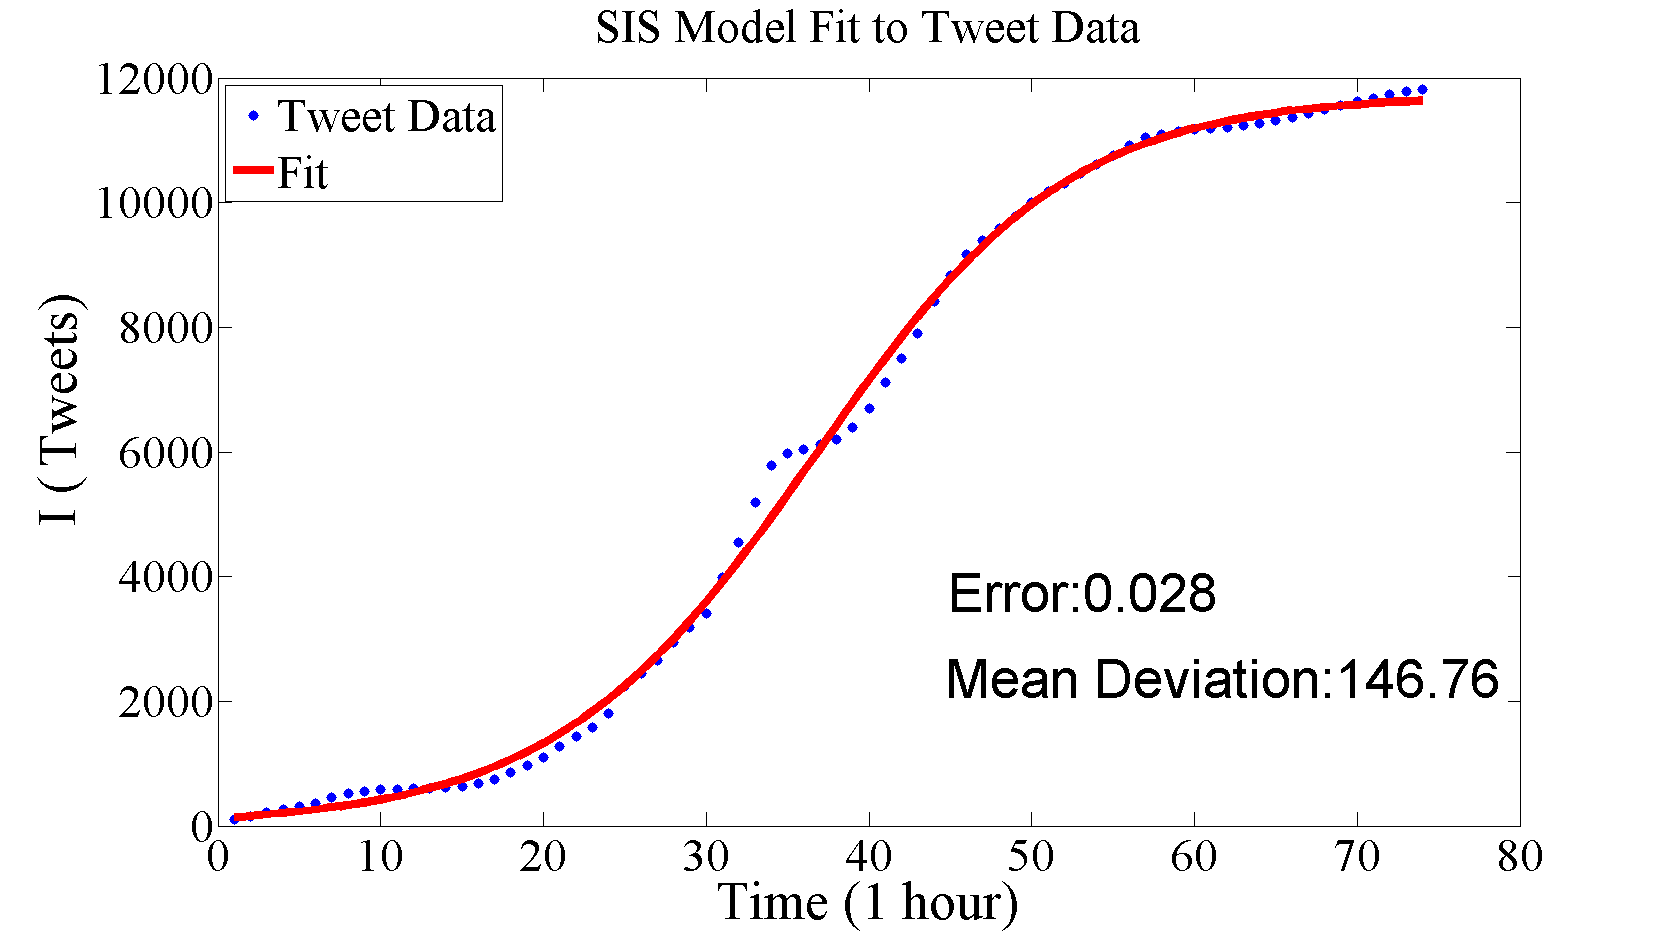
\includegraphics[width=2in,height=1.5in] {pictures/Doom_SIS.png}
   \label{fig:Doomsday_sis}
 }
   \subfigure[SEIZ]{
   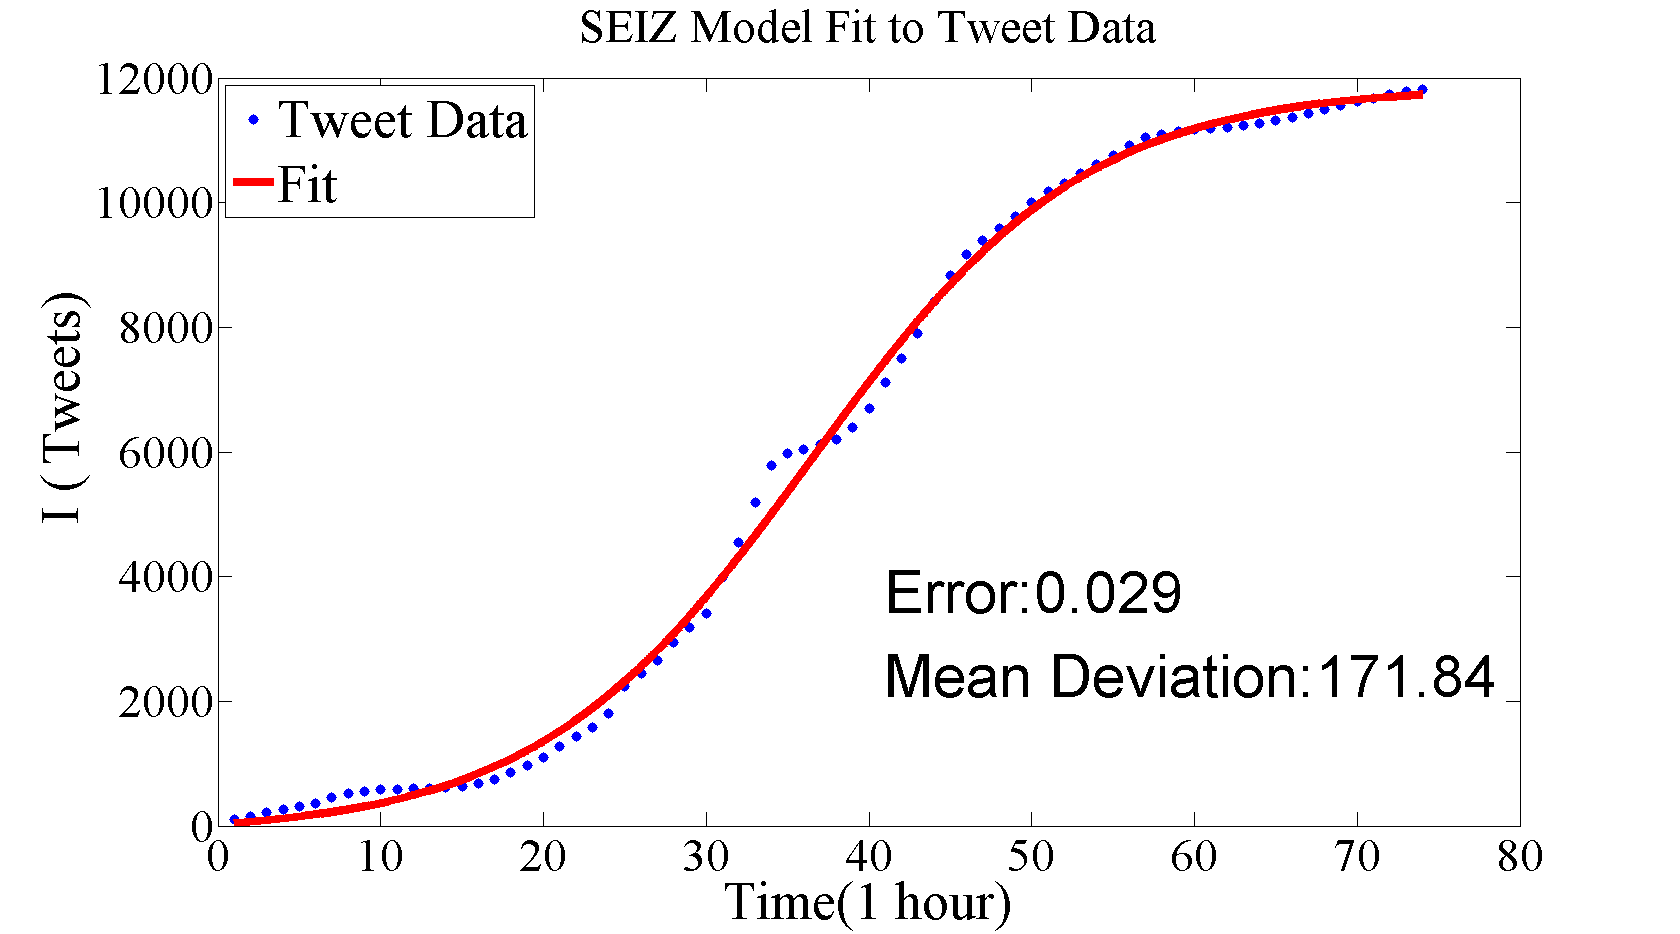
\includegraphics[width=2in,height=1.5in] {pictures/Doom_SEIZ.png}
   \label{fig:Doomsday_seiz}
 }
\vspace{-1em}
\caption{Best fit modeling for Doomsday rumor.}
\label{fig:Doomsday}
\end{figure}





\begin{table*}[t]
\tiny
\caption{Fitting error of SIS and SEIZ models}
\vspace{0.5em}
\centering
\begin{tabular}{| p{0.8cm}| p{1.2cm}| p{1cm} | p{1cm}| p{1.2cm} | p{1.3cm} | p{1.5cm} | p{1.2cm} | p{1.2cm}| p{1.3cm}| }
\hline
&\textbf{Boston}& \textbf{Pope} & \textbf{Amuay} & \textbf{Michelle} & \textbf{Obama} &\textbf{Doomsday} &\textbf{Castro}& \textbf{Riot}& \textbf{Average}   \\ [1ex]
\hline
\textbf{$SIS$} & 0.058 &0.041 & 0.058 & 0.088 & 0.102 & 0.028 & 0.082 & 0.088 & 0.068\\[1ex]
\hline
\textbf{$SEIZ$} & 0.010 & 0.004 &0.027 & 0.061 &0.101 & 0.029 & 0.073 & 0.093 & 0.050 \\[1ex]
\hline
\end{tabular}
\label{table:error} % is used to refer this table in the text
\end{table*}


Another constraint is the inability to quantify the total population size. This value appears to simply be the total number of Twitter accounts; however the value that we truly want is the number of individuals {\bf who could be exposed to the news or rumor topic}. This value shows to be very different from the total number of Twitter accounts. Consider the $\sim$175 million (M) registered Twitter accounts. Of these, (i) $\sim$90 million have no followers, and (ii) $\sim$56 million follow no one\footnote{http://www.businessinsider.com/chart-of-the-day-how-many-users-does-twitter-really-have-2011-3}. To further complicate the matter, there exists an abundance of
``fake'' Twitter accounts, which are never used by any real person. They are simply sold to users wishing to enhance their perceived popularity. Coupling these facts with sporadic Twitter usage due to night-time inactivity and user ``unplugging", it is clear that establishing a reliable estimate of users who could receive a tweet is quite difficult.

Synthesizing all of these factors, we assume the following in our SEIZ model implementation:
 %1) We do not have reliable population specifics:   		we do not know $N$, total population size; we do not know $S(t_0), E(t_0), I(t_0), $ or $Z(t_0)$,  the initial values of each population compartment. 2) Infected individuals ($I$) submit a tweet. 3) Skeptics ($Z$) have been exposed to story, but do not tweet. 4) Vital dynamics do not contribute to the overall population size. Thus, $N$ is a constant.

\begin{enumerate}
\item   We do not have reliable population specifics.
	\begin{enumerate}
    		\item We do not know $N$, total population size.
    		\item We do not know $S(t_0), E(t_0), I(t_0), $ or $Z(t_0)$,  the initial values of each population compartment.
  	\end{enumerate}
\item  {\bf Infected} individuals ($I$) submit a tweet.

\item  {\bf Skeptics} ($Z$) have been exposed to story, but do not tweet.

\item  Vital dynamics do not contribute to the overall population size. Thus, $N$ is a constant.
\end{enumerate}


The implication of these assumptions is that total population size N and initial population sizes for each compartment $S(t_0), E(t_0), I(t_0), $ and $Z(t_0)$ are viewed as unknowns. They are therefore treated as parameters in the parameter fit routine, and fit along with the other model parameters \cite{powerofgoodidea:2006}.

\subsection{Parameter Identification}

For each of the population models (SIS and SEIZ), represented by equation sets~\ref{eq:sis} and~\ref{eq:seiz}, we performed a nonlinear least squares fit of the model to Twitter data. As shown in Figure~\ref{fig:implementation_flow}, each step of this fitting process involved selecting a set of parameter values (rate constants and probabilities in equations \ref{eq:sis} and \ref{eq:seiz}, and initial compartment sizes), and numerically solving the system of ODEs with these parameter values. The set of parameter values that minimized $|I(t)-tweets(t)|$ was identified as the optimal parameter set.

The experimental implementation was done in Matlab. The {\bf lsqnonlin} function performed the least squares fit. The ODE systems were solved with a forward Euler function that we developed. This algorithm was selected due to its computational efficiency, and used a time-step of no more than 0.05. This threshold demonstrated to be numerically stable; in several instances we compared the forward Euler solution to those generated by Matlab's ode45 ($5^{th}$-order Explicit Runge-Kutta with embedded $4^{th}$-order error control), and observed nearly identical solutions.



\begin{figure}[t]
\centering
\subfigure[SIS]{
   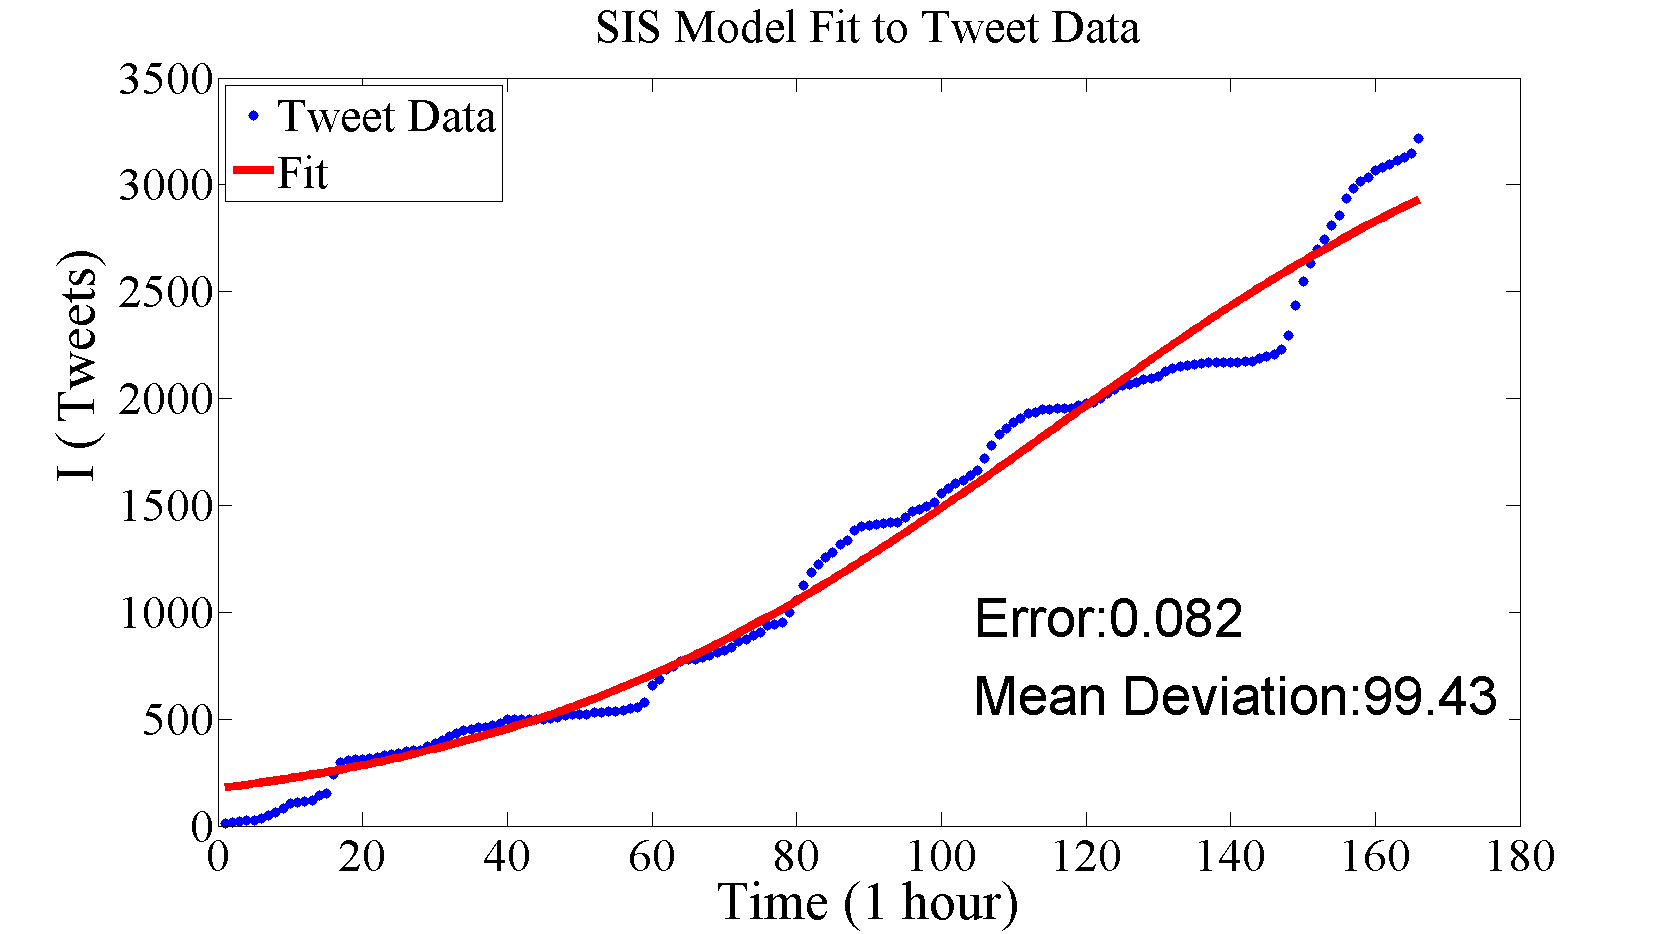
\includegraphics[width=2in,height=1.5in] {pictures/Castro_SIS.png}
   \label{fig:Castro_sis}
 }
  \subfigure[SEIZ]{
   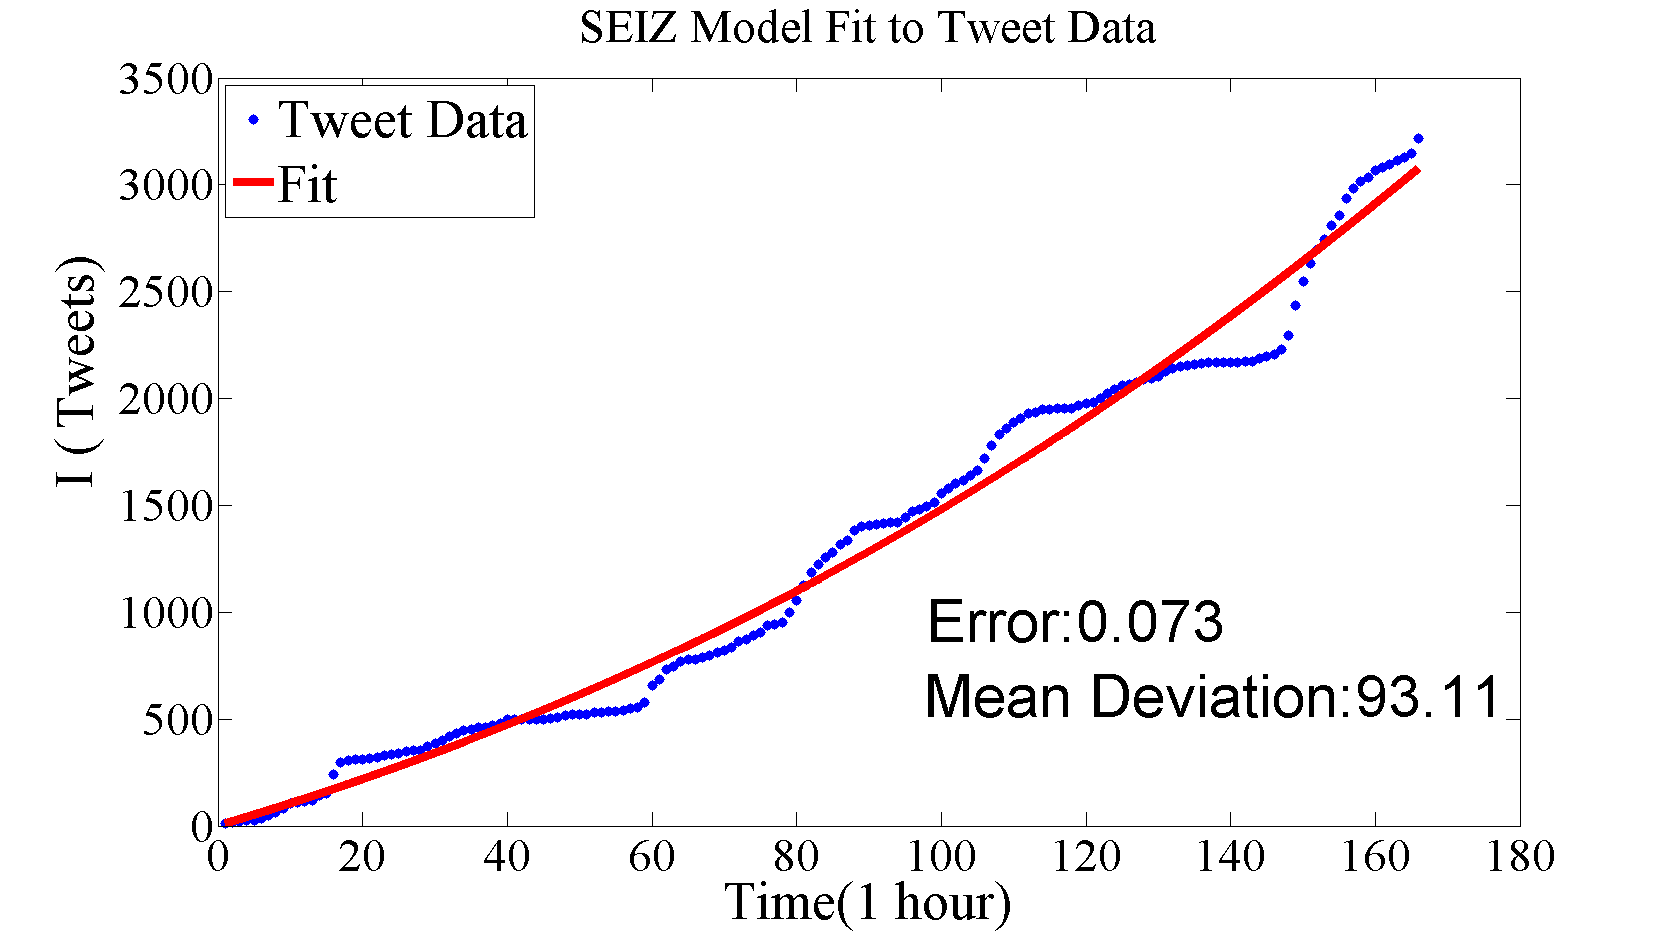
\includegraphics[width=2in,height=1.5in] {pictures/Castro_SEIZ.png}
   \label{fig:Castro_seiz}
 }
\vspace{-1.2em}
\caption{Best fit modeling for Castro rumor.}
\label{fig:Castro}
\end{figure}


\begin{figure}[t]
\centering
\subfigure[SIS]{
   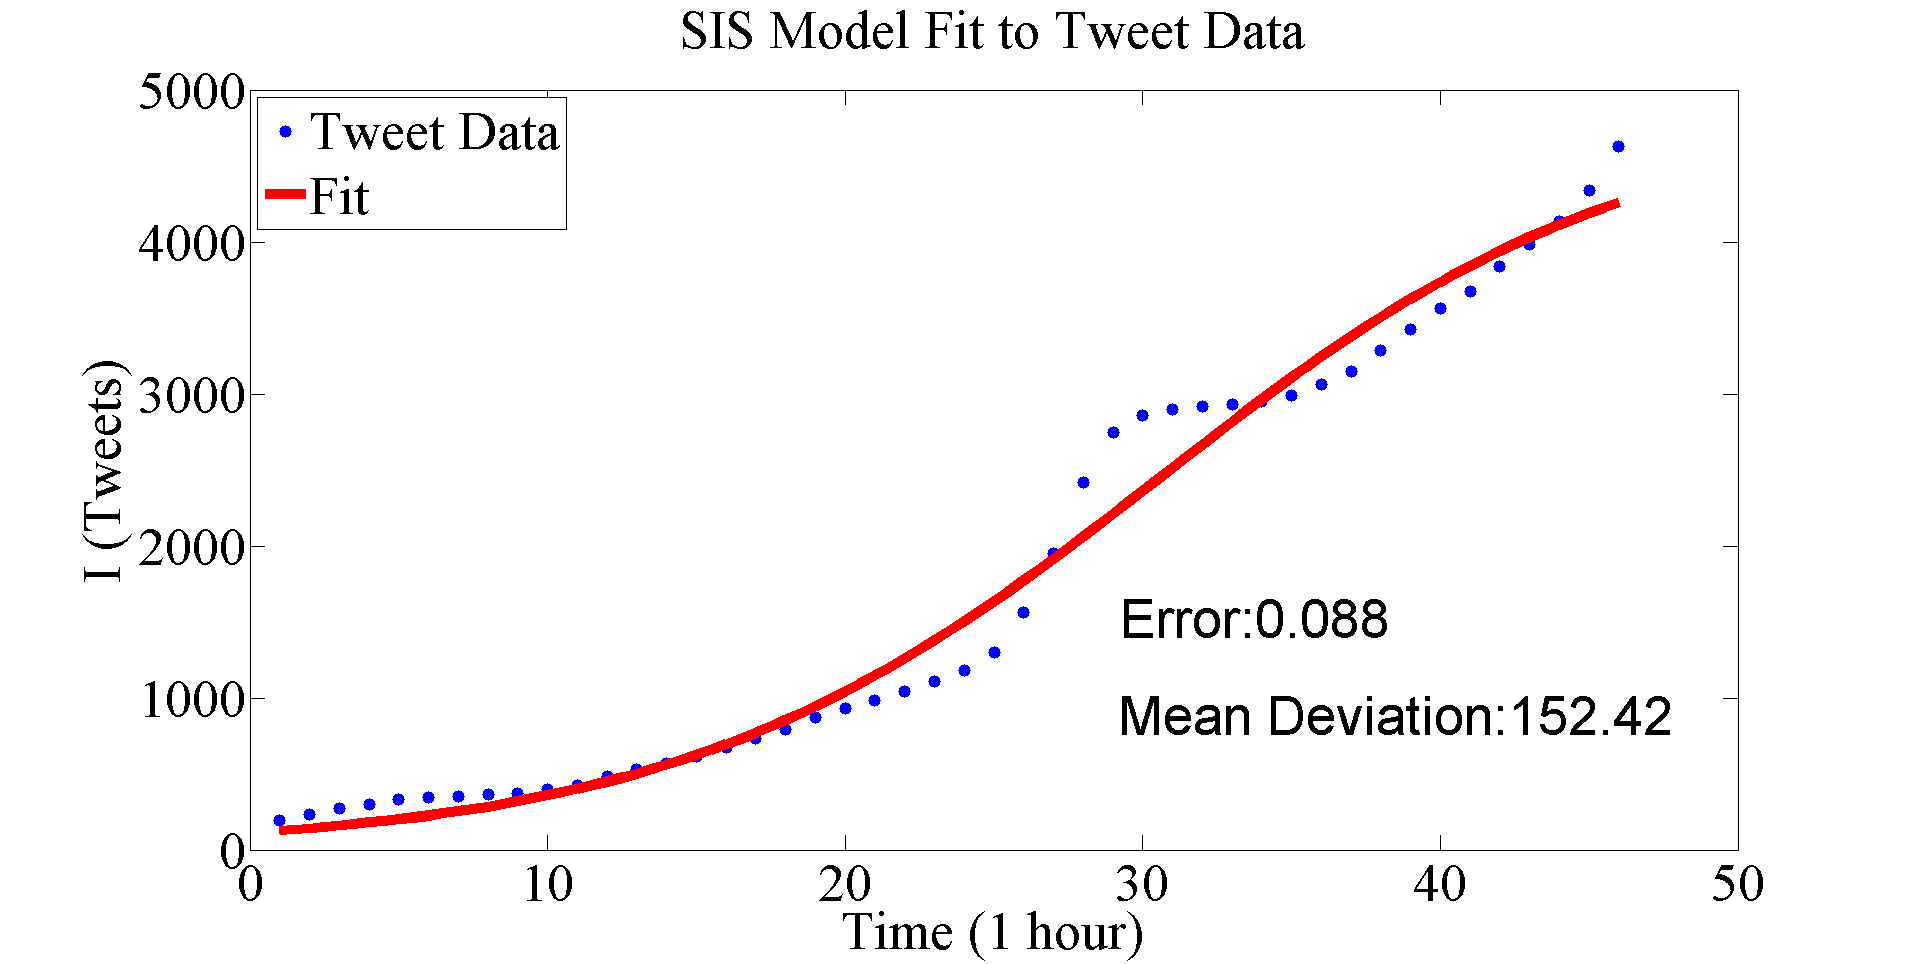
\includegraphics[width=2in,height=1.5in] {pictures/Riot_SIS.png}
  \label{fig:Mexico_riot_sis}
 }
  \subfigure[SEIZ]{
   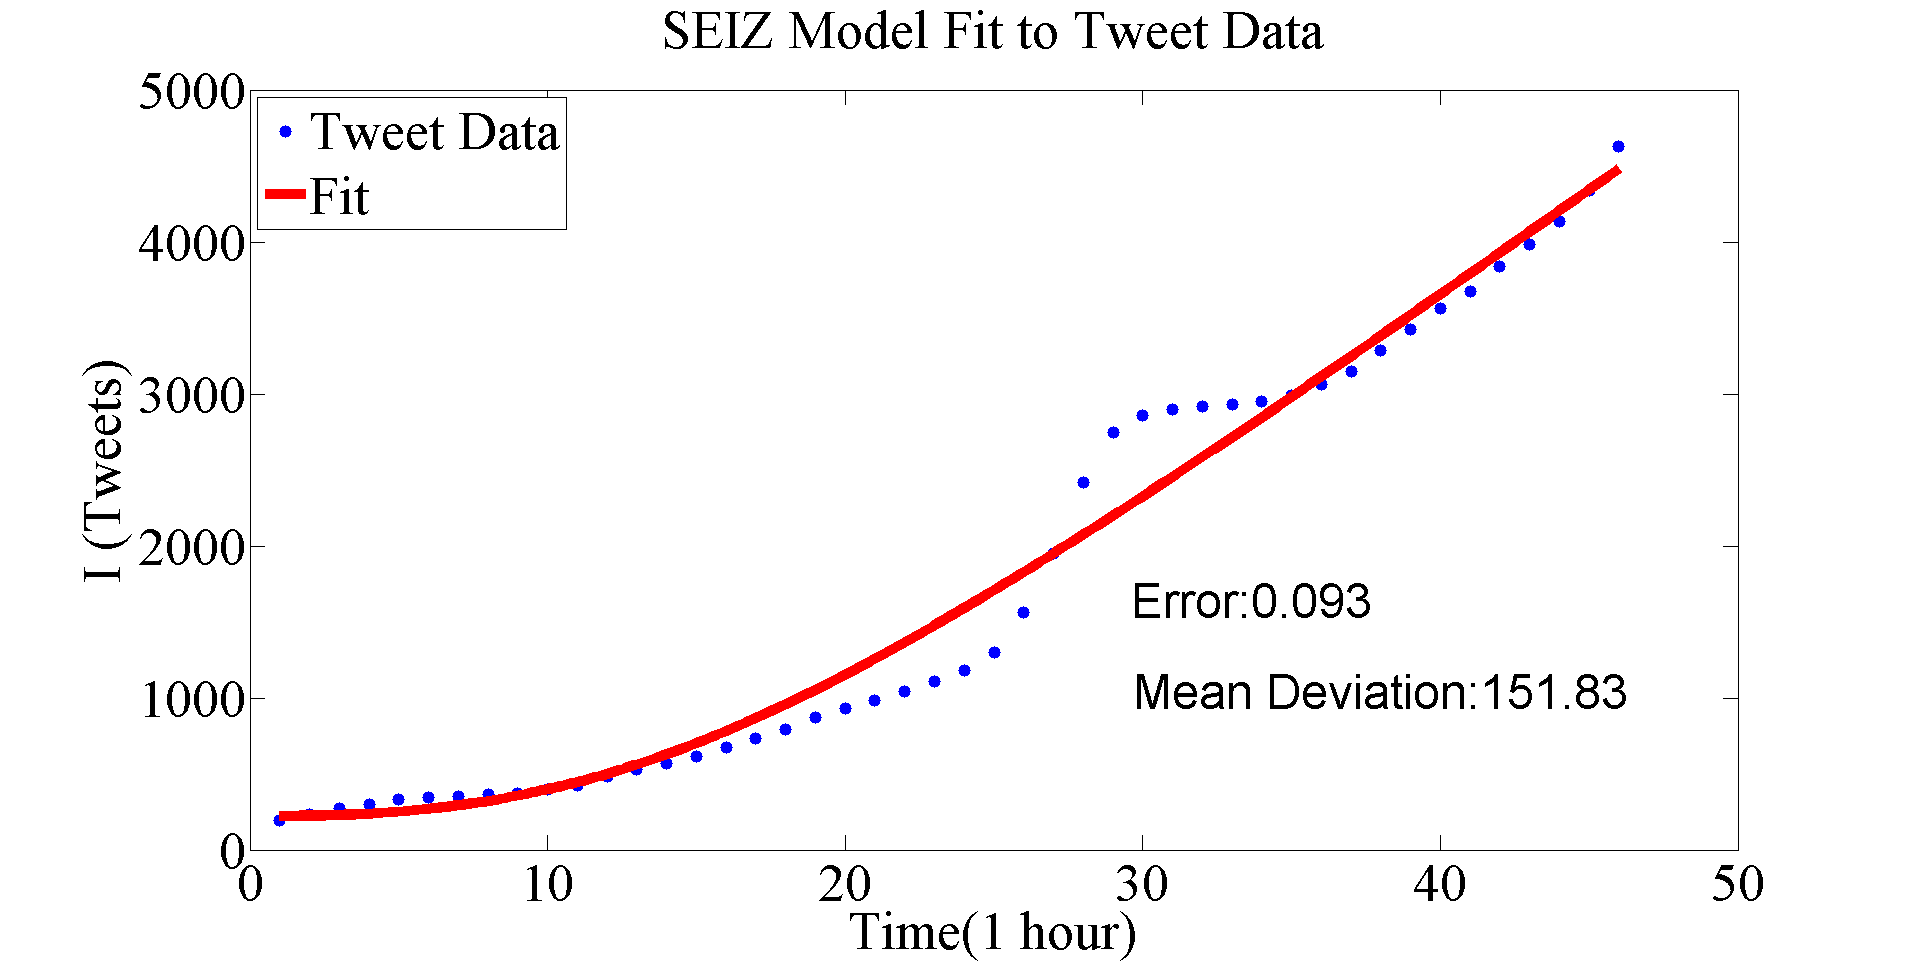
\includegraphics[width=2in,height=1.5in] {pictures/Riot_SEIZ.png}
  \label{fig:Mexico_riot_seiz}
 }
\vspace{-1.2em}
\caption{Best fit modeling for Riot news.}
\label{fig:Mexico_riot}
\end{figure}


\section{Experimental Results}
\subsection{Fitting Results}

For each of the Twitter datasets, we were interested in quantifying the transitions of users through the different compartments of the SIS and SEIZ models.
Figures~\ref{fig:Boston_bombing} -~\ref{fig:Mexico_riot} display the results for the best fit of SIS and SEIZ models (Equations~\ref{eq:sis} and~\ref{eq:seiz}) to the eight Twitter stories. Also displayed for each figure are the relative error in 2-norm $$\frac{||I(t) - tweets(t)||_2}{||tweets(t)||_2}$$ and the mean error deviation $$\frac{\sum_{i=1}^n|I(t_i)-tweets(t_i)|}{n},$$  where $n$ is the number of data points.



\begin{figure}[h]
\centering
\subfigure[Boston]{
   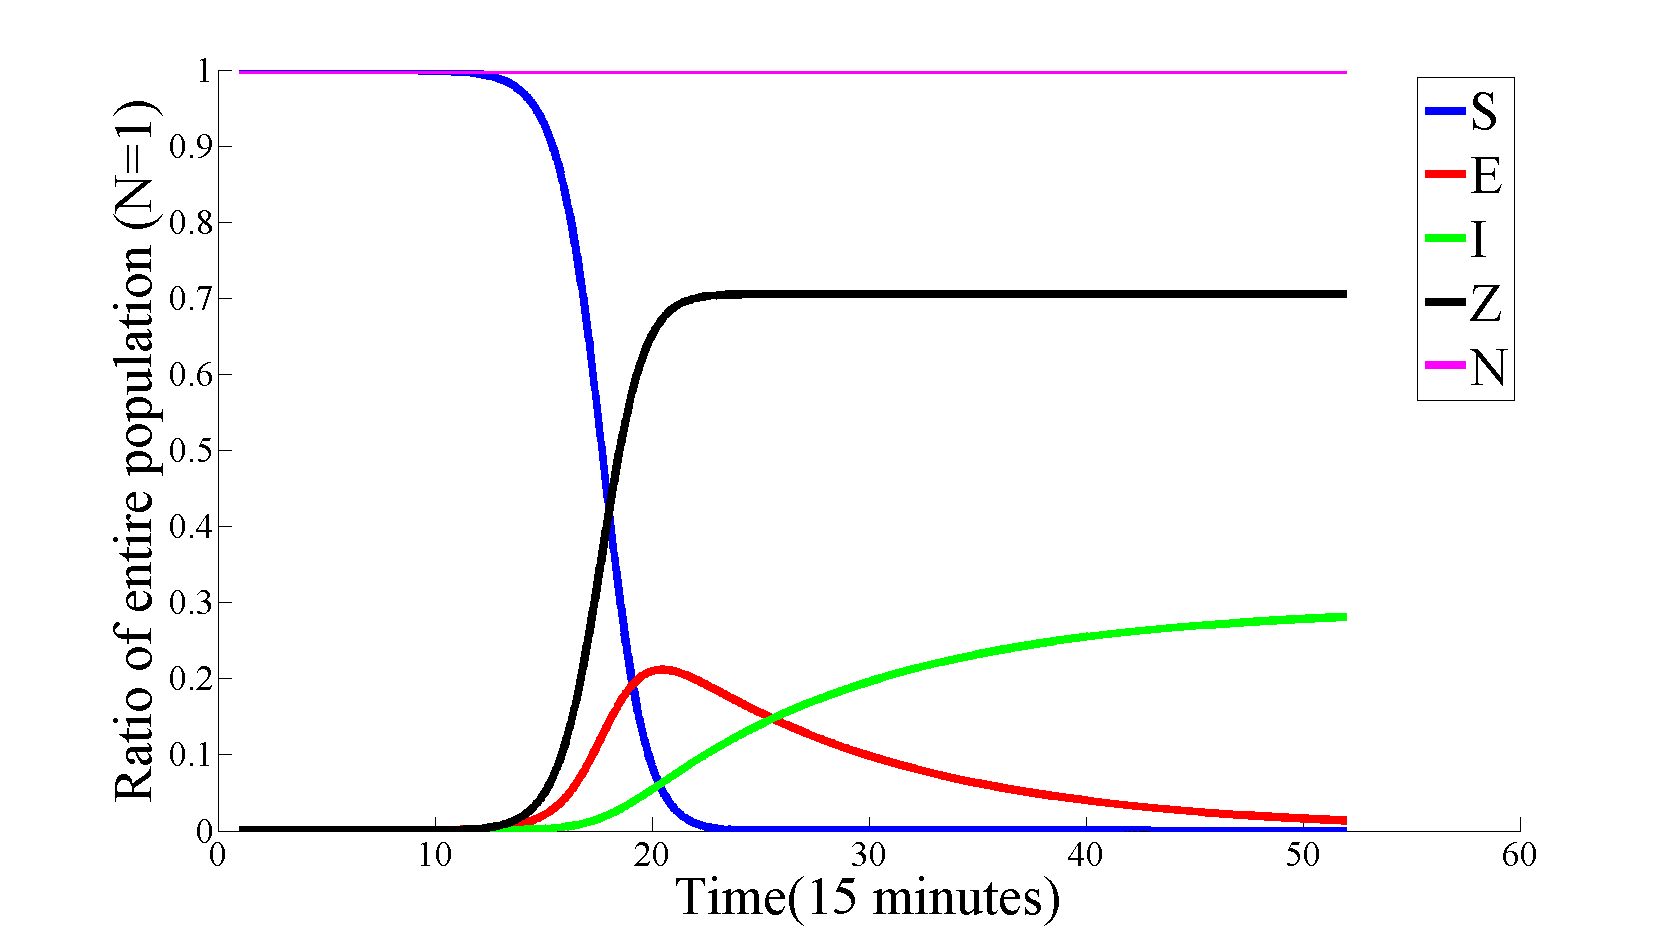
\includegraphics[width=2in,height=1.5in] {pictures/Boston_SEIZ_total.png}
  \label{fig:Boston_time}
 }
  \subfigure[Pope]{
   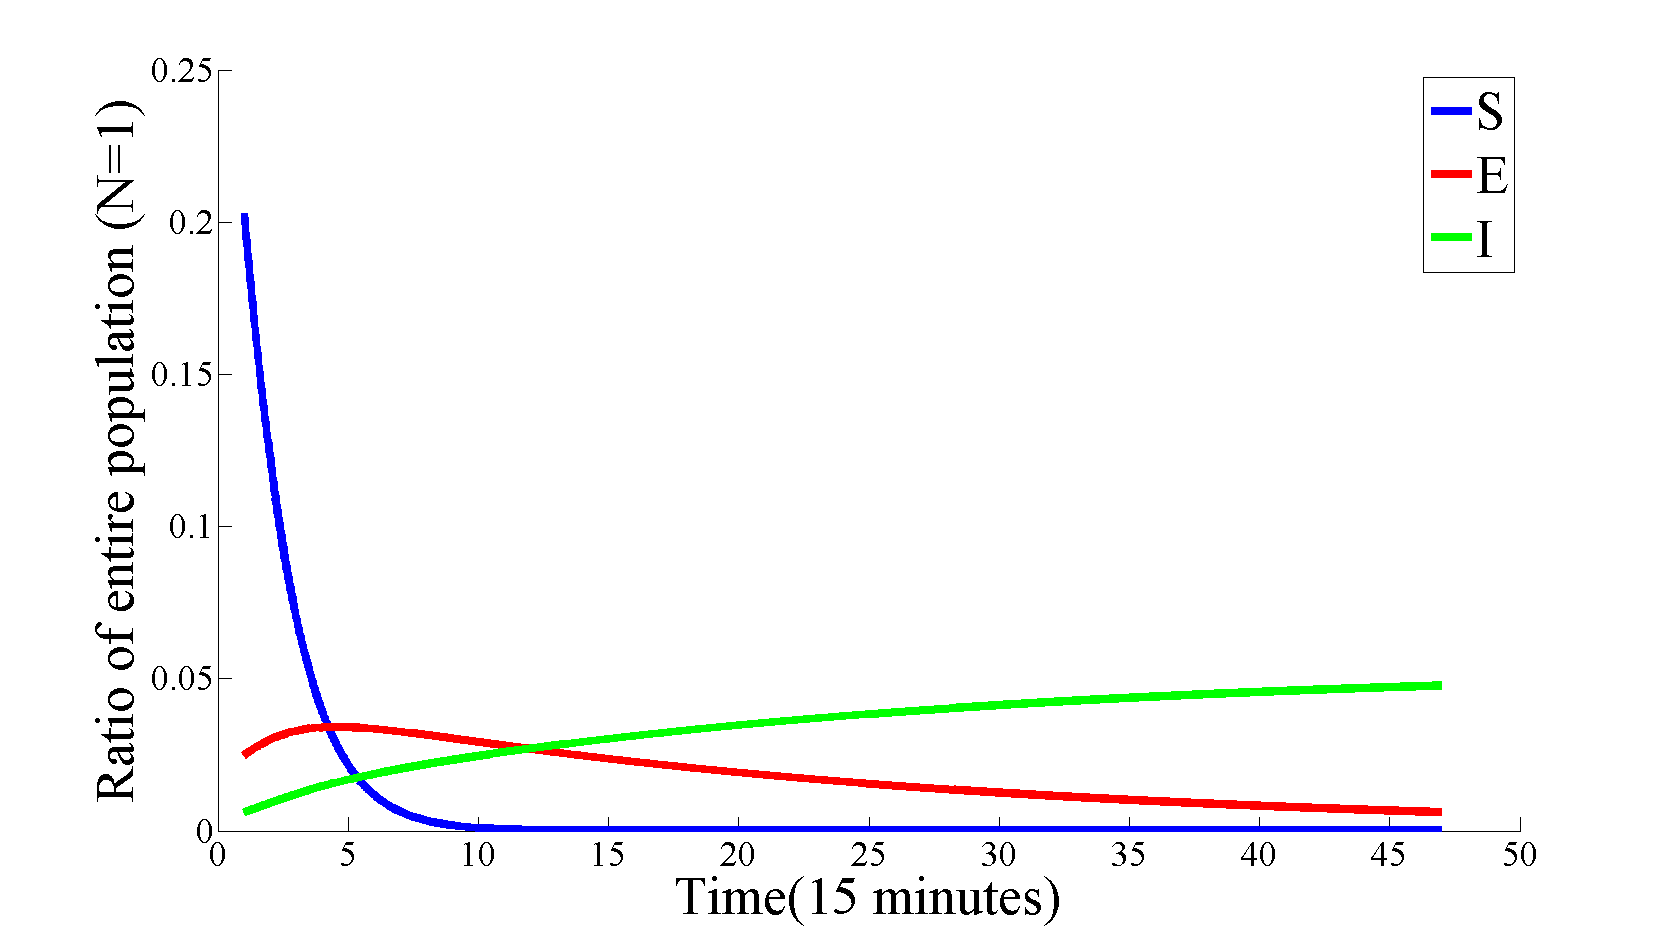
\includegraphics[width=2in,height=1.5in] {pictures/Pope_SEIZ_total.png}
   \label{fig:Pope_time}
 }
  \subfigure[Amuay]{
   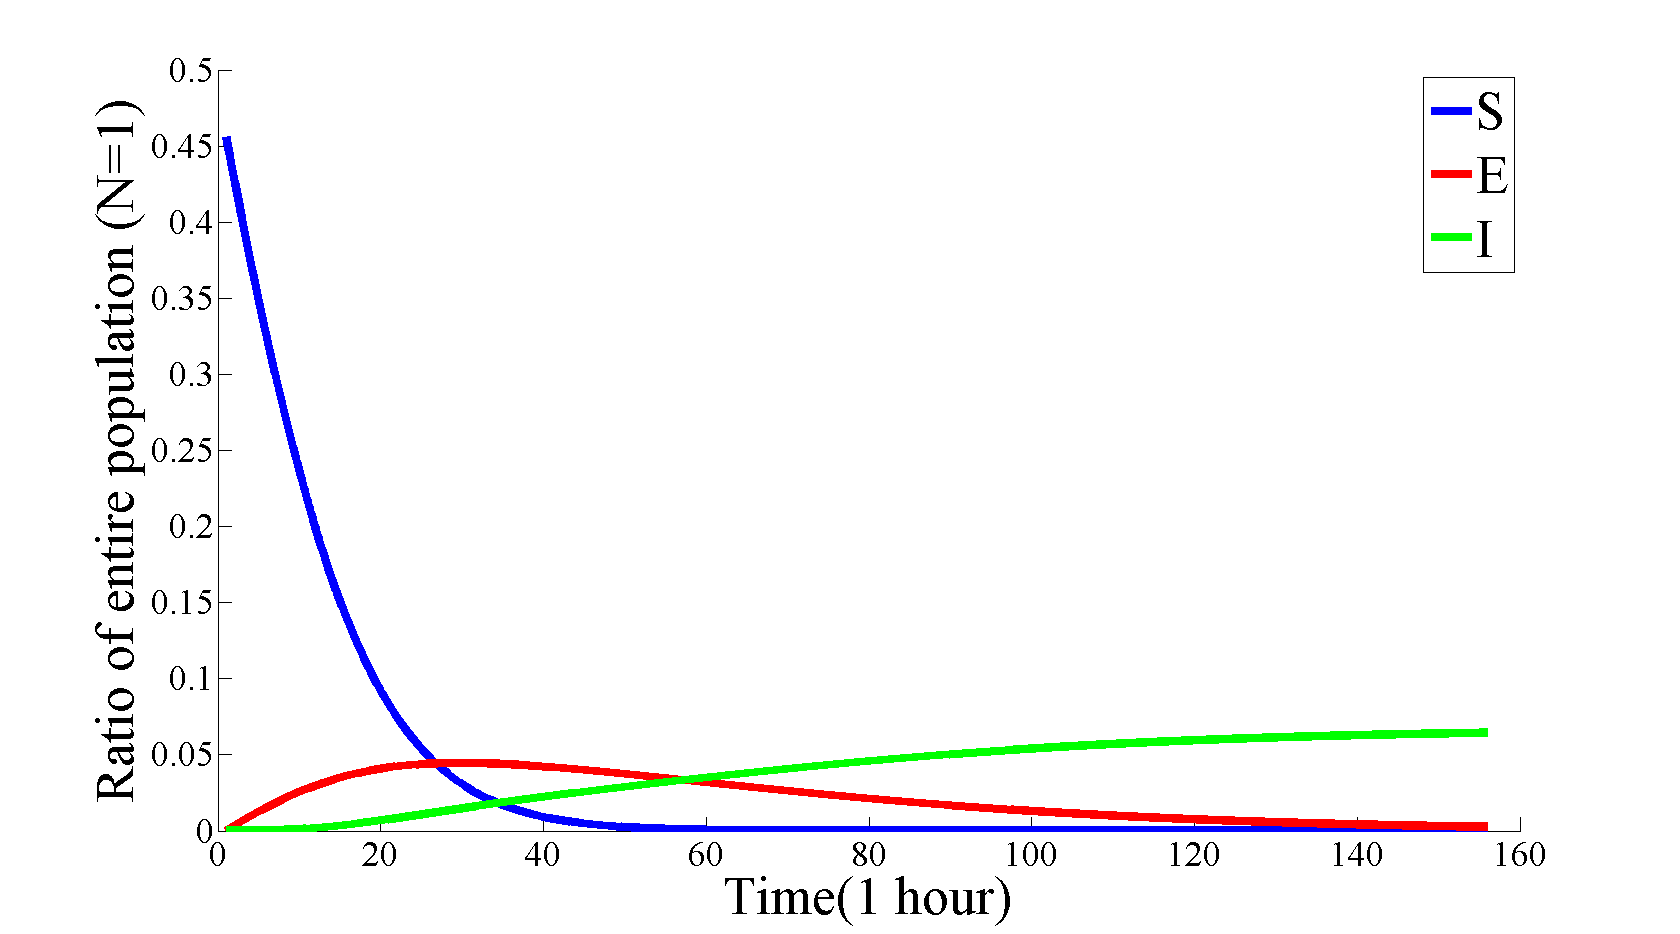
\includegraphics[width=2in,height=1.5in] {pictures/Amuay_SEIZ_total.png}
   \label{fig:Gas_time}
 }
\subfigure[Michelle]{
   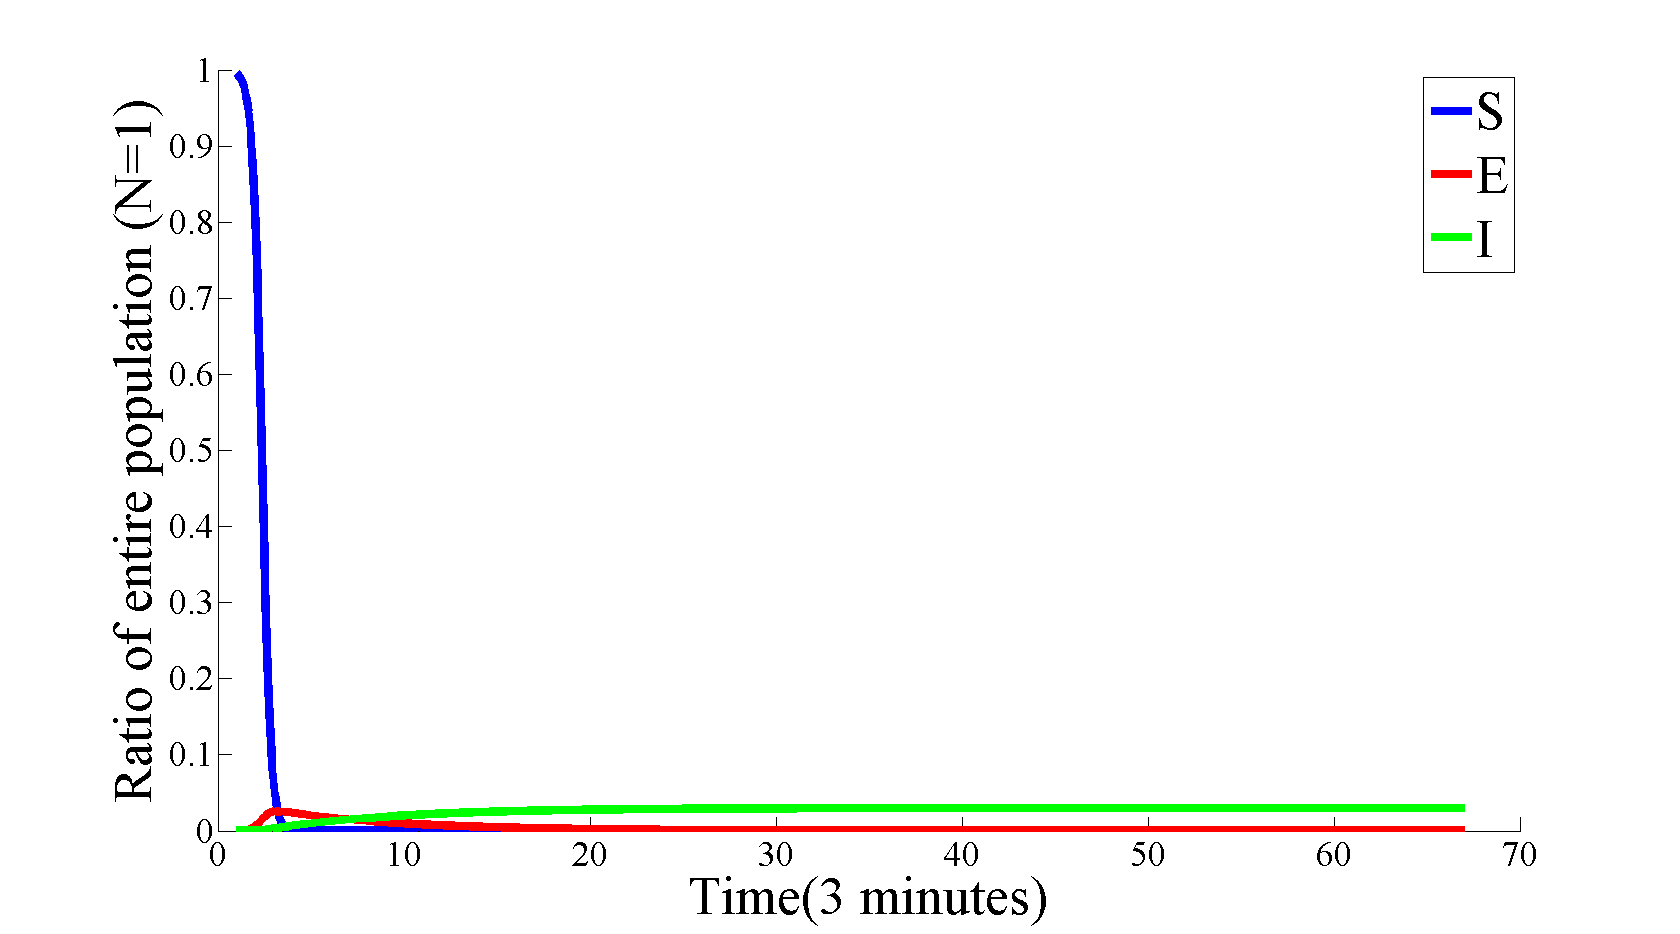
\includegraphics[width=2in,height=1.5in] {pictures/Michelle_SEIZ_total.png}
  \label{fig:Michelle_time}
 }
  \subfigure[Obama]{
   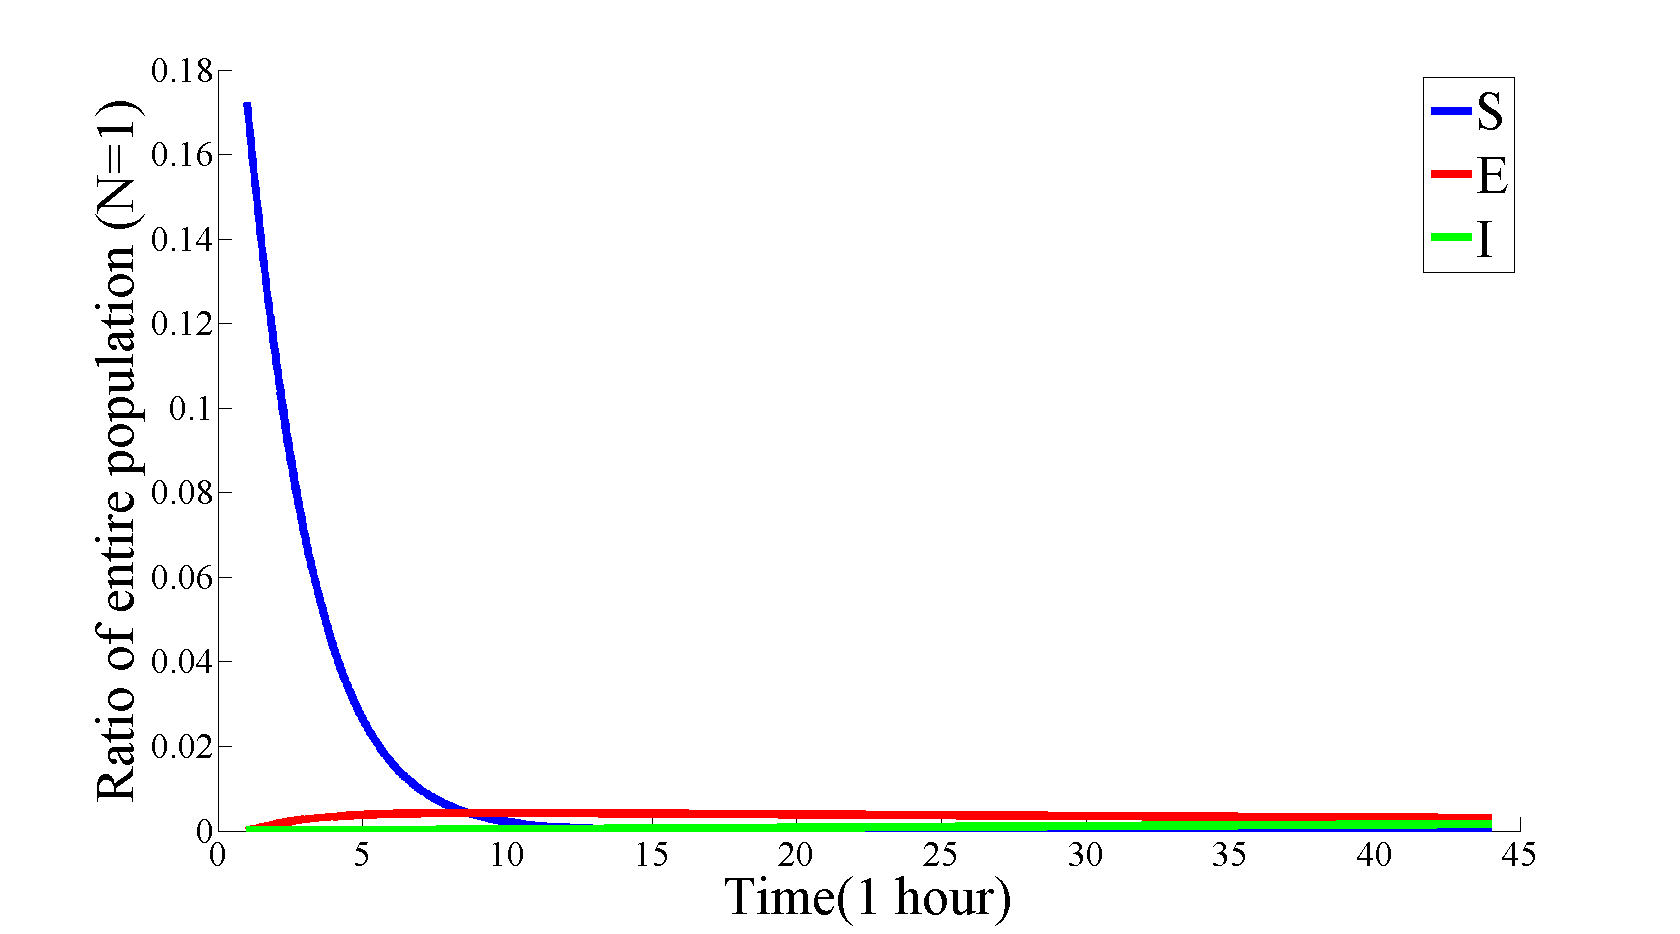
\includegraphics[width=2in,height=1.5in] {pictures/Obama_SEIZ_total.png}
   \label{fig:Obama_time}
 }
  \subfigure[Doomsday]{
   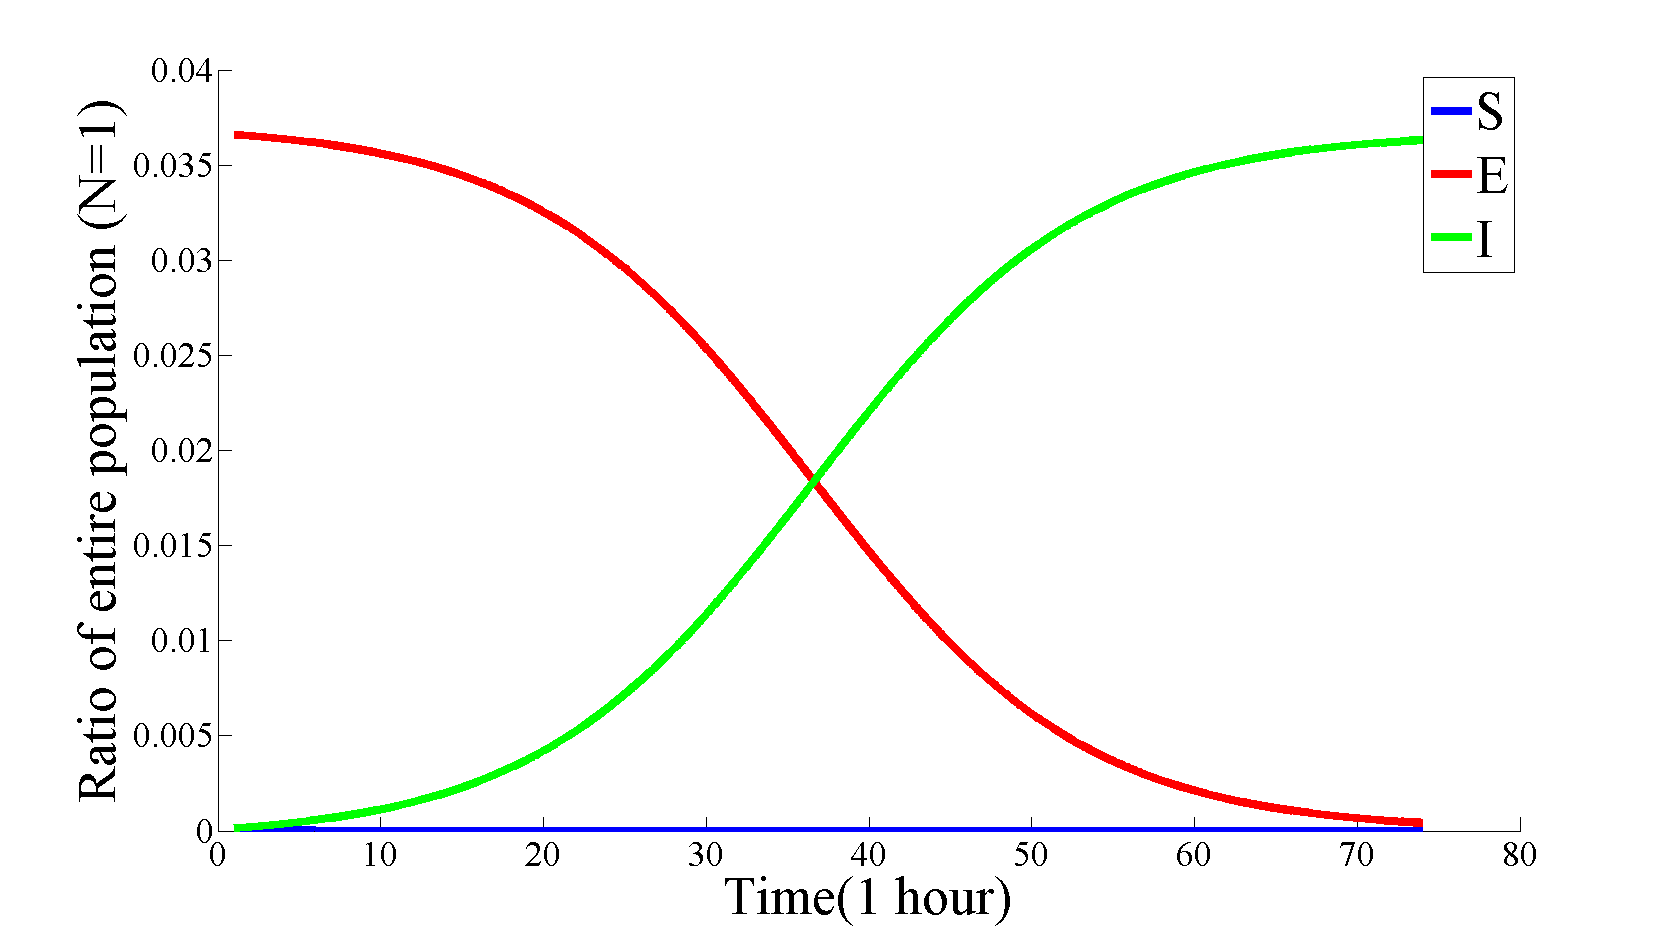
\includegraphics[width=2in,height=1.5in] {pictures/Doom_SEIZ_total.png}
   \label{fig:Doomsday_time}
 }
   \subfigure[Castro]{
   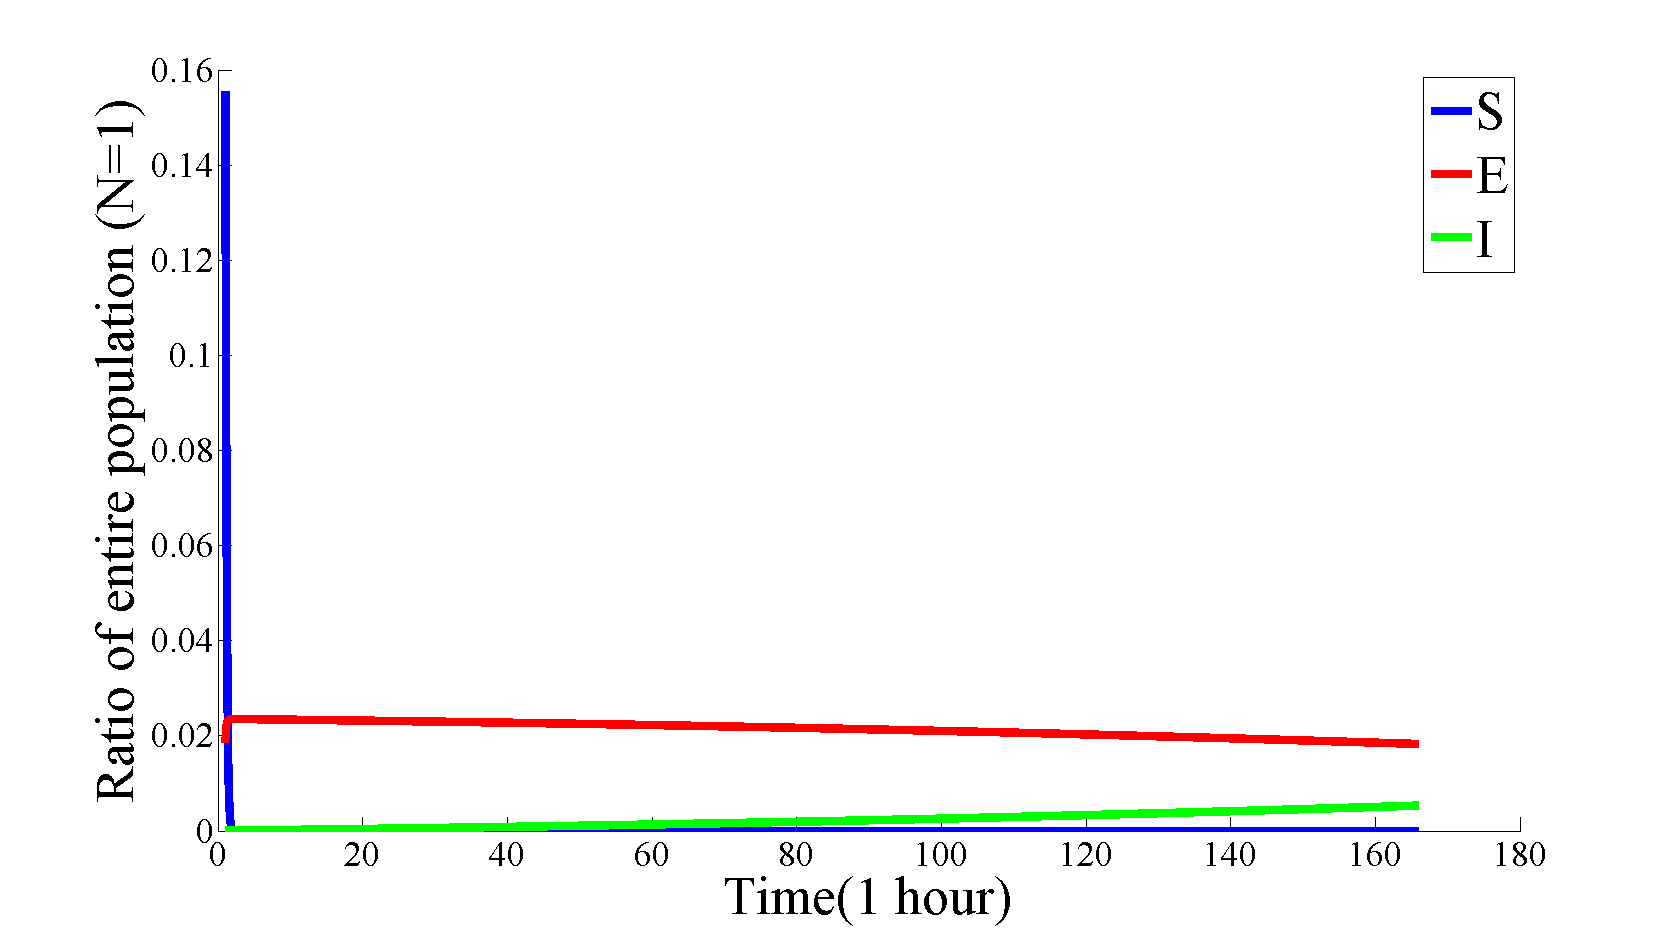
\includegraphics[width=2in,height=1.5in] {pictures/Castro_SEIZ_total.png}
  \label{fig:Castro_time}
 }
 \subfigure[Riot]{
   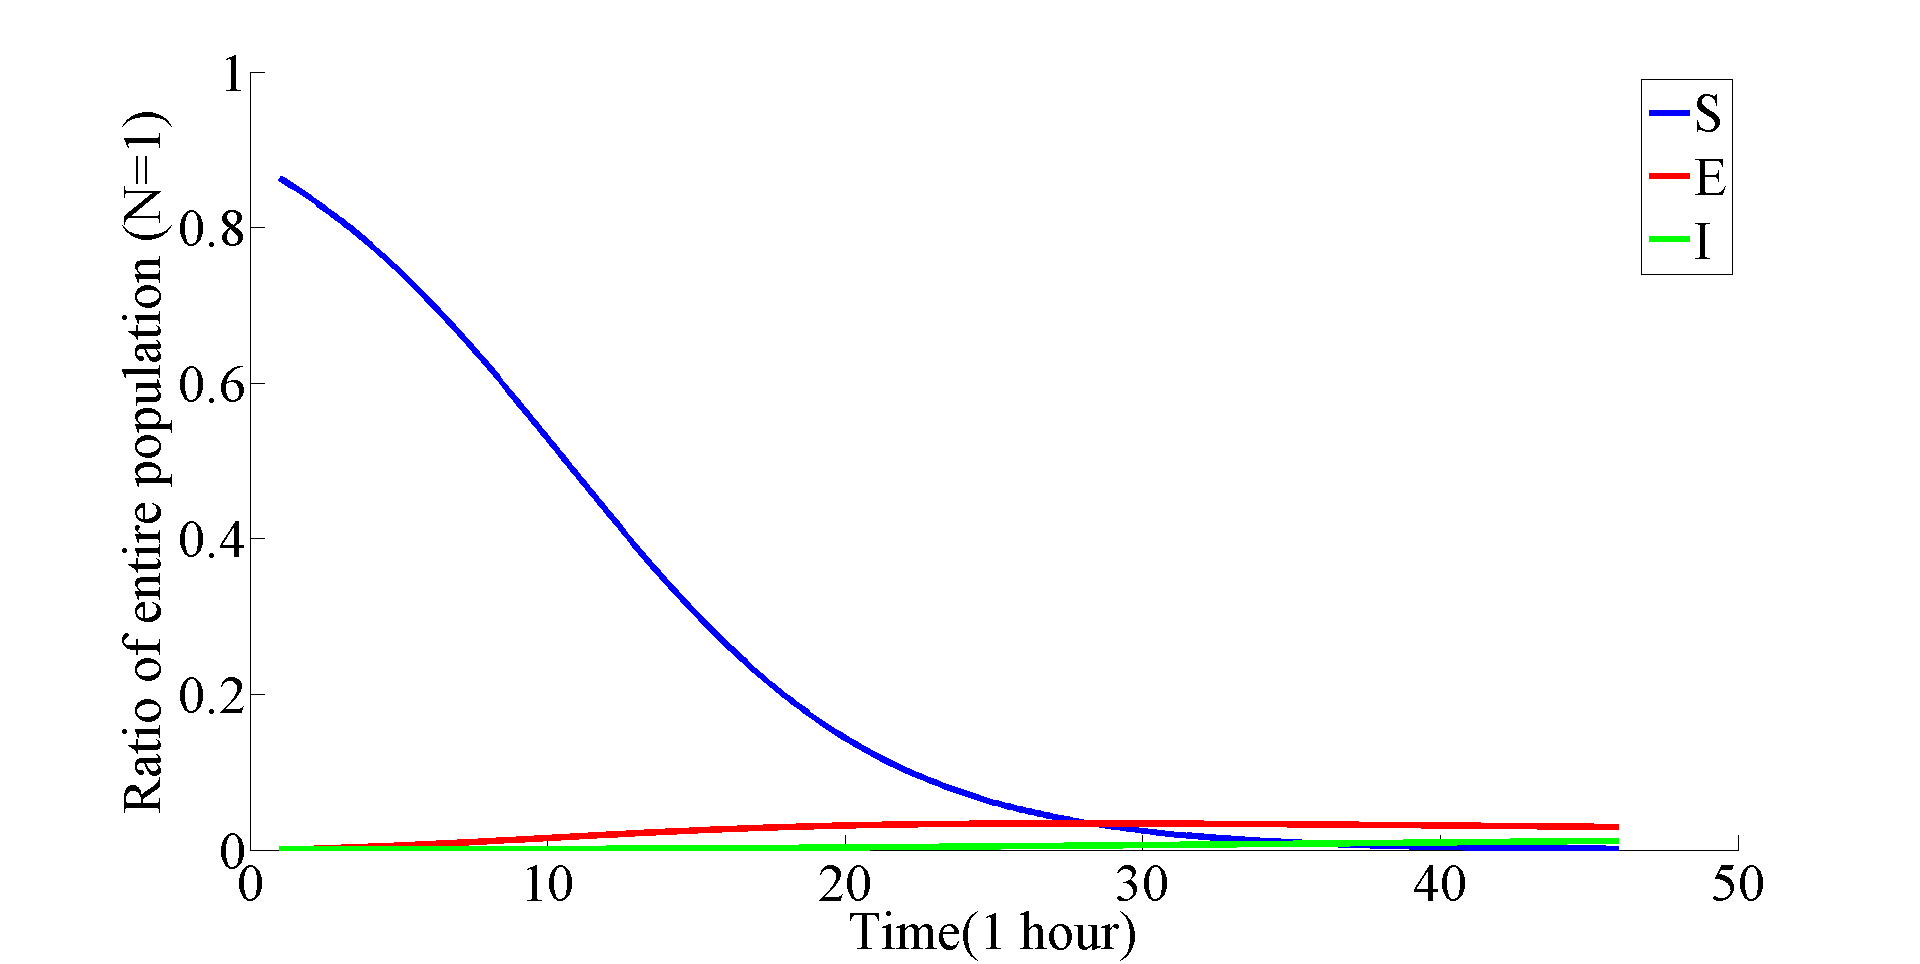
\includegraphics[width=2in,height=1.5in] {pictures/Riot_SEIZ_total.png}
  \label{fig:Mexico_time}
 }
\vspace{-0.5em}
\caption{SEIZ compartment time-course results.
\label{fig:Time_course}
}
\end{figure}


The error metrics for these eight stories clearly indicate that the SEIZ model fits the Twitter data much more accurately than the SIS model. Furthermore, the low relative error of the SEIZ model fit suggests that this model accurately represents the Twitter data for each of the eight stories; see Table~\ref{table:error}. A common observation about all the eight stories is that the SEIZ model is far more accurate in modelling the initial spread of the news on Twitter as compared with the SIS model. This behaviour can be explained by the delay caused by individuals in the ``Exposed" category taking some time before posting a story themselves~\cite{powerofgoodidea:2006}.

Given that the SEIZ model is superior to the SIS model in this application, and that the SEIZ model demonstrates an accurate representation of information diffusion on Twitter, a natural question arises ``How can this model help us?" The answer is really simple. Since we have a mathematical model for the Twitter data, we can study solutions to some of the constraints as mentioned in the ``Practical Issues" section. A well fitted SEIZ model provides values for all contact rates and transition probabilities as defined by Equation~\ref{eq:seiz}. These parameters empower us to investigate the dynamics of news and rumor spread on Twitter in a fashion that is not possible without a mathematical model. Table~\ref{table:parameters} specifies the SEIZ model parameters that we can now examine to assess news and rumor propagation on Twitter.

\subsection{Boston Marathon Bombing Analysis}

To demonstrate a line of analysis that is now possible with the SEIZ mathematical model, we use quantities from the SEIZ model fit of the Boston Marathon bombing Twitter data (Table~\ref{table:parameters}). Results are summarized in Table~\ref{tab:seiz_boston_bombing}.

Here we discuss the dynamics of all 4 compartments, so we specially show all 4 compartments in the SEIZ time-course plot only for Boston Marathon bombing (Figure~\ref{fig:Boston_time}). These results suggest that the effective rate of susceptible individuals becoming skeptics is much greater than those that becoming infected. The decrease in $S(t)$ occurs directly with an increase in $Z(t)$, and $S(t)$ becomes stable at the same time that $Z(t)$. $I(t)$ does increase as $S(t)$ decreases, but its rate of change is much slower, and the majority of $I(t)$ increase occurs after $S(t)$ has stabilized to a minimal value, demonstrating that the continued change in the infected compartment has no further influence on the change in the susceptible compartment.

Table~\ref{tab:seiz_boston_bombing} also demonstrates that the skeptics compartment is more influential on transitioning susceptible users to the exposed class than does infected users. Figure~\ref{fig:Boston_time} shows this as the increase in $E(t)$ is strongly correlated with the increase in $Z(t)$. $E(t)$ also peaks as $Z(t)$ peaks, and $E(t)$ begins to decrease at a rate negative to that of the $I(t)$ increase. In fact, the increase in $I(t)$ directly coincides with a comparable decrease in $E(t)$. These data suggest that the increase in infected users is not due in large part by recruitment of susceptible users, but rather from the natural transition to the infected compartment by exposed individuals.

Putting this all together, we can deduce that virtually all individuals are initially in the susceptible compartment. Most susceptible users become skeptics from interaction with skeptics, and those susceptible users that do transition to the exposed class do so by their interaction with skeptics. The infected compartment increases predominately from the exposed class, and not from direct recruitment of susceptible individuals. Thus, these findings suggest that it was in-fact non-Twitter mediums that most greatly aided in the generation of Twitter propagation! Further, the $\frac{\epsilon}{\rho}$ ratio indicates that the exposed users became infected more so due to information incubation and self-adoption, and not so much from direct contact with infected users.

\begin{table}
\renewcommand{\arraystretch}{2.5}
\small
\centering
\caption{Ratios of SEIZ model for Boston dataset.}
\vspace{0.5em}
\begin{tabular}{|p{2.5cm} |  p{1.5cm}|} \hline
$\displaystyle \frac{bl}{\beta p}$ & 3.1E5\\ \hline
$\displaystyle \frac{b(1-l)}{\beta (1-p)}$ & 1.0E4 \\ \hline
$\displaystyle \frac{\epsilon}{\rho}$ & 7.8\\
\hline\end{tabular}
\label{tab:seiz_boston_bombing}
\end{table}

% I added this sentence to answer review 1.4
The remaining instances of SEIZ time-course plots are shown in Figure~\ref{fig:Time_course}, we can see how S, E, and I dynamic change over time. These analyses exemplify the types of analyses that can be used to study Twitter dynamics via the SEIZ population model.

\subsection{Rumor Detection}
We next examined if our implementation of the SEIZ model, applied to our Twitter examples, could be utilized to facilitate the discrimination of true news from rumors. We began by assembling an equation to relate the key parameters of the SEIZ model. In our first attempt at performing this, we restricted our attention to the exposed compartment; this class has direct or indirect interconnections between the other three compartments, and is a key path to the infected compartment. To exemplify this, consider the extreme case where susceptible individuals are attempted to be recruited by skeptics, and ultimately end up in the infected compartment (Figure~\ref{fig:seiz-framework}). This can only be accomplished by passing through the exposed compartment.


We quantify a ratio through E as the ratio of the sum of the effective transition rates \textit{entering} this compartment (from $S$) to the sum of the transition rates \textit{exiting} this compartment (to $I$). We define this ratio as $R_{SI}$, using the subscripts to denote the contributions from the susceptible and infected compartments in this quantity:

\begin{equation}
\label{eq:R_es}
R_{SI}=\frac{(1-p)\beta +(1-l)b}{\rho + \epsilon}
\end{equation}

$R_{SI}$ possesses all rate constants and probability values of the SEIZ model and relates them to the exposed compartment with a kind of flux ratio, viz.
the ratio of effects entering E to those leaving E. A $R_{SI}$ value greater than 1 implies that the influx into the exposed compartment is greater than the efflux. Similarly, a value less than 1 indicates that members are added to the exposed group more slowly than they are removed. We hypothesized that this measure could potentially aid in the distinction of rumor topics from news topics; all parameters of the SEIZ fit are utilized in this measure, and they are related via the $R_{SI}$ value to a key compartment of this model. If a distinction between rumors and true news stories is to be seen with the SEIZ model, we identify the $R_{SI}$ measure to be a probable candidate in aiding this process.

\begin{figure}[h]
\centering
  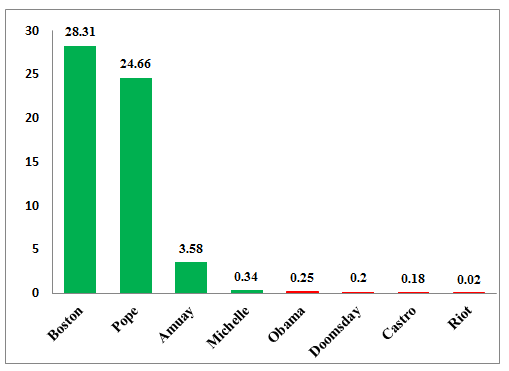
\includegraphics[width=4in]{pictures/reproductive-ratio.png}
   \caption{Ultimate $R_{SI}$ values for eight Twitter datasets.}
  \label{fig:static_ratio}
\end{figure}


\paragraph{Ultimate $R_{SI}$ value}
We then computed $R_{SI}$ using the specific parameter values attained from our model fits of the eight cases (Figure~\ref{fig:static_ratio}).
Here we can see that the true news about the Boston Marathon bombing, Pope resignation, and Amuay refinery explosion do in fact have much higher $R_{SI}$ values than the rumor topics: Doomsday, Fidel Castro death, Mexico City riots, and Barrack Obama injury which each have much lower $R_{SI}$ values. However, the Michelle presence at the Oscars, which is classified as true news, has a very low $R_{SI}$ value. This particular case is interesting since Michelle did not really show up to the 2013 Oscar Awards Ceremony. She simply participated remotely via video telecast. It is thus arguable that this topic could have been discussed in the media in terms similar to rumors.

\paragraph{Dynamic $R_{SI}$ value}

\begin{figure}[h]
\centering
  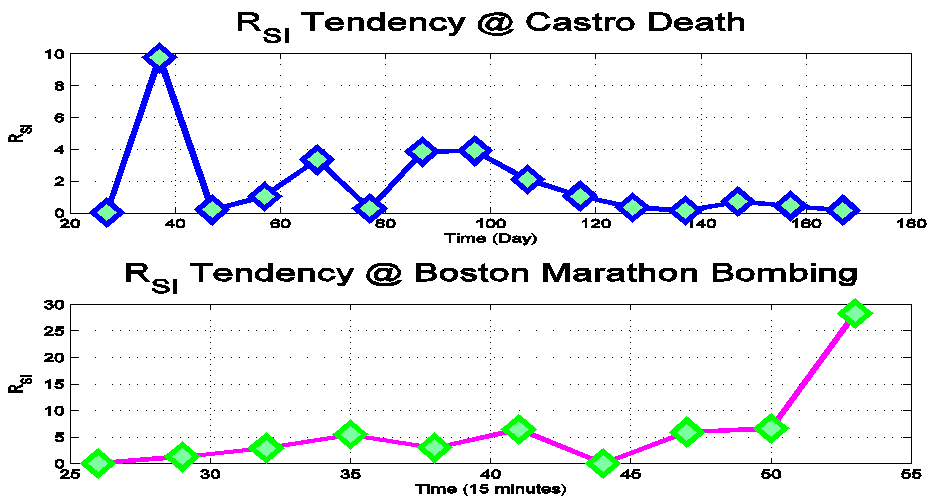
\includegraphics[width=4.5in]{pictures/Castro-Boston-realtime-RSI.png}
   \caption{Dynamic $R_{SI}$ values for Castro rumor and Boston bombing real news.}
  \label{fig:dynamic_castro_ratio}
\end{figure}

For one story, if we collect related Tweets at the very beginning stage, then the $R_{SI}$ value would be a time series. Figure~\ref{fig:dynamic_castro_ratio} shows the dynamic $R_{SI}$ values for Castro rumor and Boston bombing real news. We can see for the Castro rumor, at the beginning stage, the $R_{SI}$ value was pretty high, which indicate considerable people believe this story. With time pass by, the $R_{SI}$ values decreased sharply. However, for the Boston Marathon bombing real news, the $R_{SI}$ value was very low at beginning, but increased rapidly within several hours and reached around 28.31 very soon. The $R_{SI}$ time series indicate people's confidence with those stories is dynamically changing.


These findings suggest, for these specific topics, that the parameters in the SEIZ model can potentially aid in the challenge of distinguishing rumor versus true news. We are not claiming that the $R_{SI}$ value is the unique measure to accomplish this, nor are we claiming that the SEIZ model itself is the sole tool to do this. As is suggested by our findings, we postulate that a fit of a compartmental model, in the spirit of the SEIZ model, to Twitter data provides valuable propagation information that can be coupled with other data analysis strategies  (e.g., content modeling)
to augment the accuracy and reliability of true news story and rumor topic discrimination.


\section{Conclusion}
In this chapter, we have demonstrated how true news and rumor stories being propagated over Twitter can be modelled by epidemiologically-based population models. We have shown that the SEIZ model, in particular, is accurate in capturing the information spread of a variety of news and rumor topics, thereby generating a wealth of valuable parameters to facilitate the analysis of these events. We then demonstrated how these parameters can also be incorporated into a strategy for supporting the identification of Twitter topics as rumor or news. As of now, we are modeling propagation over static data. In future, we plan to adapt this model for capturing news and rumors in real-time.

%In this chapter, we have quantified information propagation, including both news or rumors,
%on Twitter using epidemic models.
%We have demonstrated that the SEIZ model is accurate in capturing
%information diffusion, especially in the initial portion of the curve.
%Using the SEIZ model, we have developed a method to detect rumors.
%In the future, we plan to incorporate more detailed follower information in
%our models, to determine exactly how many twitter users receive
%tweets from a sender.
%Such data can be used to determine SEIZ transition rates more accurately.
%Another interesting approach that we plan to explore in the  future
%is to use sentiment analysis on tweets to analyze whether an individual is
%a skeptic or infected or just exposed. Finally, we would like to develop
%an automated method to separate rumors from truth using a multiplicity of features.





\endgroup
